\chapter{AdaptaMaterialEscolar 2.0}
\label{cap:AdaptaMaterialEscolar2.0}
En este capítulo explicaremos la obtención de requisitos y cómo se han clasificado en la Sección \ref{cap:requisitos}. También se describirá el diseño realizado por cada integrante de la aplicación para la iteración competitiva y el diseño final de las funcionalidades en la Sección \ref{disenyoDeLaAplicacion}. Por últimmo, en la Sección \ref{sec:implmentaction} se expondrá cómo se ha implementado la aplicación.

\section{Requisitos}
\label{cap:requisitos}

Lo primero que hicimos fue analizar la memoria de AdaptaMaterialEscolar 1.0 \citep*{AdaptaMaterialEscolar1.0} extrayendo las funcionalidades que faltaban por implementar y los resultados de la evaluación que se realizó. Tras este análisis decidimos agrupar las funcionalidades que habría que incluir en la nueva versión de la aplicación según los datos sobre los que trabajan y las acciones que realizan. De esta forma han surgido las siguientes agrupaciones: formato (funcionalidades que tienen relación con el estilo o la estructura del documento), ejercicios (funcionalidades relacionadas con la creación de actividades) y auxiliar (resto de funcionalidades que no pertenecen a formato o a ejercicios). Siguiendo esta estructura las funcionalidades quedan agrupadas de la siguiente manera:
\\

\begin{itemize}
  \item Funcionalidades relacionadas con el formato:
        \begin{itemize}
          \item Añadir encabezado al texto: El usuario eligirá un encabezado que se añadirá al documento de trabajo.
          \item Añadir un tipo de fuente escolar: Incluir en los tipos de fuentes la escolar. Dicha fuente se refleja en la Figura \ref{escolar}.
                \begin{figure}[ht!]
                  \centering
                  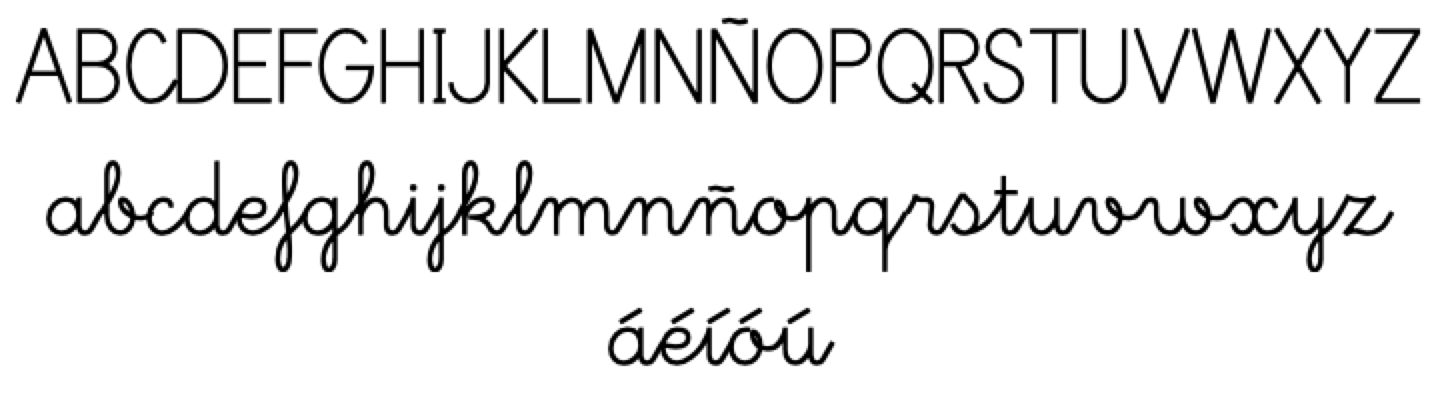
\includegraphics[scale=0.3]{AdaptaMaterialEscolar/FunteEscolar.png}
                  \caption{Fuente escolar.}
                  \label{escolar}
                \end{figure}
          \item Añadir una leyenda de colores: Sirve para que el docente pueda poner de distintos colores distintas palabras según la categoría a la que pertecenecen, por ejemplo sustantivos en rojo y adjetivos en verde.
          \item Añadir leyenda de colores para el tema de cada asignatura: Dar la posibilidad de que cada asignatura tenga un color. Al crear un documento según la asignatura se pondrá el borde del documento del color que corresponde a dicha asignatura.
          \item Añadir cuadrícula: En vez de renglones de una única línea se podrá poner para responder a una pregunta la cuadrícula.
          \item Añadir la opción de añadir doble pauta: En vez de renglones de una única línea se podrá poner para responder a una pregunta la doble pauta.
          \item Estandarizar formato para títulos e índices del temario: Dar la opción de crear estilos para estandarizar el documento de trabajo.
          \item Enumerar ejercicios de forma automática: Establecer un orden numérico para los ejercicios de forma automática según se van creando para que el usuario no se tenga que preocupar de ese aspecto.
        \end{itemize}

  \item Funcionalidades asociadas con la creación de ejercicios:
        \begin{itemize}
          \item Ejercicios de relacionar contenido mediante flechas: Generar un ejercicio para relacionar conceptos mediante flechas.
          \item Añadir ejercicios de cálculo con huecos a rellenar por el alumno: Posibilidad de introducir ejercicios de cálculo con espacios en blanco para que el alumno rellene dichos huecos con contenido adecuado.
          \item Añadir ejercicios con espacio para dibujar: Añadir amplio hueco en blanco con el fin de que el alumno pueda dibujar.
          \item Ejercicios de completar los espacios en blanco en tablas y esquemas: Dada una tabla o un esquema se establecen espacios en blanco para que el alumno los rellene con el contenido adecuado.
        \end{itemize}

  \item Funcionalidades auxiliares:
        \begin{itemize}
          \item Generar un resumen a partir de un texto.
          \item Exportar el documento a formato Word.
          \item Añadir un pictotraductor que permita dada una frase traducirla a pictogramas.
          \item Añadir imágenes buscando una palabra: A partir de una palabra se busca su respectiva imagen en las bases de datos de imágenes libres.
          \item Sustituir una palabra por una imagen: Dado un texto esta funcionalidad permitirá que se seleccione una palabra, se busque una imagen asociada a dicha palabra y esta se reemplazará por la imagen seleccionada.
          \item Crear una herramienta de recorte de imágenes: Tras seleccionar una imagen se dará la opción de quitar partes de la misma.
          \item Crear tablas que organicen el temario y/o las actividades, seleccionando contenido: Tras la selección de contenido por parte del usuario se creará una tabla en base a la información seleccionada, con un formato predefinido.
          \item Creación de esquemas.
        \end{itemize}

\end{itemize}

Tras haber analizado en detalle las funcionalidades anteriores hemos encontrado que varias de ellas ya están implementadas en la versión original de AdaptaMaterialEscolar y otras hemos decidido no implementarlas actualmente ya que consideramos que no tenemos la información suficiente para ello, pero las realizaremos una vez podamos reunirnos con los usuarios finales y obtener más información sobre ellas. El resto de funcionalidades son las que implementaremos en este proyecto.

Las siguientes funcionalidades son las que ya están implementadas en la versión original:
\begin{itemize}
  \item Añadir encabezado al texto: El documento de trabajo tiene una opción con una lista de encabezados para añadir uno y cuando se pulsa un encabezado el documento de trabajo convierte el formato de la letra en el del encabezado seleccionado.
  \item Enumerar ejercicios de forma automática: El documento de trabajo permite añadir listas enumeradas.
\end{itemize}

Las funcionalidades que hemos decidido descartar de momento por falta de información son las siguientes:
\begin{itemize}
  \item Añadir imágenes buscando una palabra. Partimos de que debemos usar una base de datos de imagen libre pero no tenemos la información suficiente para definir cuál sería la base de datos correcta.
  \item Sustituir una palabra por una imagen. No la realizaremos ya que no tenemos claro de dónde obtener las imágenes ni el estilo de estas.
  \item Crear una herramienta de recorte de imágenes para el texto original: No la realizaremos ya que no tenemos claro qué tipo de recorte tenía pensado el usuario.
  \item Crear tablas que organicen el temario y/o las actividades, seleccionando contenido: Descartamos dicha funcionalidad ya que no tenemos la información suficiente del formato que desea el usuario.
  \item Crear esquemas: Descartamos dicha funcionalidad ya que no tenemos la información suficiente del formato que desea el usuario.
  \item Ejercicios de completar los espacios en blanco en tablas y esquemas. Descartamos esta funcionalidad ya que depende de la funcionalidad de crear tablas y esquemas.
\end{itemize}

Por lo tanto, las funcionalidades que vamos a implementar son las que se muestran a continuación:

\begin{itemize}
  \item Generar un resumen a partir de un texto con el fin de ayudar a un alumno a comprender los elementos claves del texto de manera mas rápida.
  \item Exportar el documento a formato Word para hacer modificaciones y que el usuario pueda continuar con las modificiones del documento.
  \item Añadir un pictotraductor con el fin de trasformar un texto a su equivalente en pictogramas para que el alumno pueda adquirir nuevos conocimientos de forma más sencilla.
  \item Ejercicios de relacionar contenido mediante flechas ya que ayuda al alumno a consolidar conceptos.
  \item Añadir un tipo de fuente escolar con el fin de facilitar la lectura y la escritura al alumno.
  \item Añadir una leyenda de colores con la categoría de cada tipo con el fin de  ayudar al alumno a relacionar conceptos.
  \item  Añadir ejercicios de cálculo con huecos a rellenar por el alumno para que el alumno practique el cálculo.
  \item  Añadir ejercicios con espacio para dibujar con el fin de que el alumno pueda reflejar lo que piensa, interpreta y representa sobre algo.
  \item Añadir leyenda de colores para el tema de cada asignatura con el fin de que el alumno pueda distinguir entre las asignaturas.
  \item Añadir cuadrícula para escribir los números con el fin de facilitar los ejercicios de matemáticas.
  \item Añadir la alternativa de añadir doble pauta con el fin de que el alumno adquiera un tamaño de letra adecuado.
  \item Estandarizar formato para títulos e índices del temario con el fin de que el profesor pueda definir un estilo.

\end{itemize}

\section{Diseño de la aplicación}
\label{disenyoDeLaAplicacion}
Analizando la interfaz de AdaptaMaterialEscolar 1.0 hemos llegado a la conclusión de que la experiencia de usuario no era cómoda. Por ejemplo, obligaba a cargar un PDF y las funcionalidades se abrían en una ventana bastante pequeña. Además, la selección de colores no nos pareció la adecuada y el estilo general de la aplicación no era moderno. Por todo lo anterior decidimos rediseñar la aplicación.

Para el rediseño hemos realizado una iteración de diseño competitiva. Esta trata de la creación, por parte de cada integrante, de un nuevo diseño de la aplicación y la puesta en común de los diseños para debatir sobre qué sería lo óptimo e intuitivo para el usuario. Luego junto a las tutoras realizamos un \textit{brainstorming} basándonos en dichos diseños. Por último, construimos el diseño final de la aplicación.

A continuación, se explicará el diseño de la aplicación por parte de cada integrante y el diseño final de la aplicación.
\subsection{Diseño de los integrantes}
En esta sección se explicará los diseños creados por cada integrante junto a las imágenes de los mismos. Todos los diseños mencionados se encuentran en los Apéndices \ref{ape:disenyoAlvaro}, \ref{ape:disenyoDunia}, \ref{ape:disenyoAlberto} y \ref{ape:disenyoJohan}.

\subsubsection{Álvaro Gómez Sittima}
\label{sec:iterAlvaro}
Para empezar, se diseñó la página de inicio la cual dispone de un menú superior con el logo de la aplicación a la izquierda y enlaces a las distintas páginas de la aplicación (Ayuda y Contacto) a la derecha. En la Figura \ref{fig:disenyoAlvaro01} se muestra el diseño de esta página. Este menú superior aparecerá en todas las páginas de la aplicación y se utilizará el logo de la aplicación como enlace a la página de inicio. En esta página el usuario podrá cargar un fichero PDF y utilizar un editor de documentos para poder adaptar el material del PDF. El acceso a las opciones de archivo, formato y adaptaciones se encontrarán como botones integrados en la barra de herramientas del editor de documentos. Además, se mostrarán opciones relevantes en un barra de herramientas flotante encima del texto que tenga seleccionado en el PDF o en el editor de documentos. El diseño de esta página sin un PDF cargado se puede ver en la Figura \ref{fig:disenyoAlvaro01a} y con un PDF cargado en la Figura \ref{fig:disenyoAlvaro01b}. Si el usuario pulsa el enlace de ayuda en el menú superior, este le llevará a la página de ayuda la cual dispondrá de un buscador con el que podrá buscar información sobre un tema en concreto, relacionado con el uso de la aplicación. Si no se realiza una búsqueda aparecerán todos los temas sobre los que se ofrece ayuda. Cada tema aparecerá en una tarjeta con información sobre el tema y un breve video para apoyar lo explicado en el texto.

En cuanto a las funcionalidades, se realizarón los siguientes diseños:
\begin{itemize}
  \item \textbf{Generar resumen}: En caso de que el usuario tenga texto seleccionado, cuando pulse la opción de generar resumen le saldrá una pequeña ventana encima con un campo para introducir el número de palabras del resumen y un botón para generar el resumen, llevándolo al documento de trabajo. En la Figura \ref{fig:disenyoAlvaro02} se muestra el diseño de esta funcionalidad en caso de tener texto seleccionado. En caso de no tener texto original, se abrirá una ventana aparte donde el usuario podrá escribir el texto a resumir y resumirlo.
  \item \textbf{Pictotraductor}: En caso de que el usuario tenga texto seleccionado, cuando pulse la opción de pictotraductor se traducirá automáticamente el texto a pictogramas y se llevará al documento de trabajo. Si pulsa alguno de los pictogramas generados podrá cambiarlo por otro. En la Figura \ref{fig:disenyoAlvaro03} se muestra el diseño de esta funcionalidad en caso de tener texto seleccionado. En caso de no tener texto original, se abrirá una ventana aparte donde el usuario podrá escribir el texto y traducirlo.
  \item \textbf{Definir huecos}: En caso de que el usuario tenga texto seleccionado, cuando el usuario pulse la opción de definir huecos, se llevará automáticamente el texto al documento de trabajo y el usuario podrá definir los huecos seleccionando las palabras. En la Figura \ref{fig:disenyoAlvaro04} se muestra el diseño de esta funcionalidad en caso de tener texto seleccionado. En caso de no tener texto original, se abrirá una ventana aparte donde el usuario podrá escribir el texto y definir los huecos.
  \item \textbf{Buscar pictograma}: Cuando el usuario pulse la opción de buscar pictogramas en la barra de herramientas del editor, se abrirá una ventana modal con un buscador. Al pulsar el botón de buscar, se mostrarán todos los pictogramas relacionados con el texto introducido, debajo del buscador. El usuario podrá arrastrar los pictogramas que desee al documento de trabajo. En la Figura \ref{fig:disenyoAlvaro05} se muestra el diseño de esta funcionalidad.
  \item \textbf{Ejercicio de definiciones}: Cuando el usuario pulse la opción de crear ejercicio de definiciones en la barra de herramientas del editor, se creará un recuadro en el documento de trabajo donde el usuario podrá añadir los distintos conceptos a definir y el número de renglones de cada definición. Cuando haya terminado de crear el ejercicio podrá darle al botón de aceptar para que el ejercicio se inserte en el documento de trabajo. En la Figura \ref{fig:disenyoAlvaro06} se muestra el diseño de esta funcionalidad.
        % \item \textbf{Sopa de letras}: Cuando el usuario pulse la opción de crear sopa de letras en la barra de herramientas del editor, se creará un recuadro en el documento de trabajo donde el usuario podrá definir el número de filas, el número de columnas y añadir las palabras a buscar en la sopa de letras. Cuando haya terminado de crear la sopa de letras podrá darle al botón de aceptar para que se inserte en el documento de trabajo.
        % \item \textbf{Leyenda de colores}: Cuando el usuario pulse la opción de crear la leyenda de colores en la barra de herramientas del editor, se creará un recuadro en el documento de trabajo donde el usuario podrá añadir los distintos conceptos y asignarles un color, con un selector de colores, a cada uno. Cuando haya terminado de crear la leyenda podrá darle al botón de aceptar para que se inserte en el documento de trabajo.
\end{itemize}

\subsubsection{Dunia Namour Doughani}
\label{sec:duniaIter}
El diseño inicial de la página principal incluye una cabecera con el logo de la aplicación, un menú desplegable que contiene las funcionalidades y un botón que te redirige a la vista de ayuda. En la parte izquierda se encuentra el documento de trabajo, mientras que la zona derecha se divide en dos secciones, una para incluir la funcionalidad seleccionada por el usuario y otra para insertar un archivo PDF, ambas con la opción de ajustar el tamaño de la ventana. Este diseño se puede visualizar en la Figura \ref{dunia1} Con respecto a las funcionalidades, he realizado los siguientes diseños:
\begin{itemize}
  \item \textbf{Generar un resumen:} El diseño de esta funcionalidad consta de un recuadro en el que introduces el texto y al pulsar un botón se genera el resumen. Para incluirlo en el documento de trabajo el usuario tendrá que darle a la opción de copiar y pegarlo en el documento de trabajo. Este diseño se puede ver en la Figura \ref{dunia2}.
  \item \textbf{Pictotraductor:} Este diseño consta de un recuadro donde introduces el texto y al darle a un botón se genera la traducción del texto a pictogramas. Para introducir los pictogramas en el documento de trabajo se hará mediante la tecla CTRL + click arrastrar al documento de trabajo los pictogramas escogidos o arrastrando todos a la vez sin seleccionar ninguno. Este diseño se puede ver en la Figura \ref{dunia3}.
  \item \textbf{Ejercicio de flechas:} Para este diseño se visualizaran dos tablas. Cada tabla tendría un botón de añadir o eliminar filas y aquellas celdas que quedasen vacías se trasformarían en huecos. Al darle al botón de terminar se incluiría el ejercicio de tablas sin el borde de estas en el documento de trabajo, donde se encuentre el puntero. Este diseño se puede ver en la Figura \ref{dunia4}.
  \item  \textbf{Leyenda de colores:} Este diseño consta de un rectángulo donde pones las palabras de la leyenda, y al lado de la palabra hay una opción para seleccionar el color. Además, dispone de dos botones, uno para añadir más palabras y otro para eliminarlas. Una vez el usuario haya finalizado la leyenda de colores pasa a colocarse. Al final del documento de trabajo, en el lado derecho. Este diseño se puede ver en la Figura \ref{dunia5}.
  \item  \textbf{Ejercicios de cálculo con huecos:} Este diseño dispone de una opción para elegir el tamaño de la expresión matemática, una vez elegido se muestra tanto huecos como el tamaño escogido, al darle a cada hueco se podrá escribir tanto un número como una operación aritmética elemental, al finalizar se incluirá la expresión matemática en el documento de trabajo donde se encuentre el puntero. Este diseño se puede ver en la Figura \ref{dunia6}.
  \item  \textbf{Leyenda de colores para el tema de cada asignatura:} Al darle a esta opción se abrirá un menú con las asignaturas, y al presionar sobre una asignatura el borde del documento de trabajo pasará a tener el color predeterminado de dicha asignatura.
\end{itemize}

Los rediseños para las funcionalidades implementadas en AdaptaMaterialEscolar 1.0 no se realizaron ya que no se encontró una manera de mejorar el diseño.

\subsubsection{Alberto Alejandro Rivas}
\label{sec:albertoIter}
En este caso, los diseños fueron realizados con la herramienta de diseño de interfaces de usuario Figma, con el objetivo de poder obtener un resultado más detallado y tener en cuenta la paleta de colores.

Se ha intentado mantener la misma estructura y funcionalidad que en la aplicación existente, pero haciendo que la interfaz de usuario sea más profesional. Para esto se ajustó el diseño de la barra de navegación, los botones, el componente para seleccionar un fichero pdf, etc. En la pantalla principal hay una barra de navegación y un componente en el que se puede arrastrar o seleccionar un fichero pdf. Una vez seleccionado el archivo, se muestra otra página que se divide en dos, en una mitad está el pdf y en la otra está el editor de texto. Estos diseños se pueden observar en las figuras \ref{AlbertoPaginaPrincipal1} y \ref{AlbertoPaginaPrincipal2}. Por último, el usuario podrá acceder a cada funcionalidad haciendo click en los botones que se encuentran en la parte superior del editor.

Para hacer el diseño de las funcionalidades ya implementadas en AdaptaMaterial 1.0 también se ha utilizado la misma estructura, haciendo algunos ajustes para darles un estilo más profesional, pero manteniendo el mismo funcionamiento. En las figuras \ref{Alberto13}, \ref{Alberto14}, \ref{Alberto15}, \ref{Alberto16} y \ref{Alberto17} se muestran los diseños de estas funcionalidades.

A continuación se muestran los diseños de las nuevas funcionalidades que no estaban implementadas en AdaptaMaterial 1.0:

\begin{itemize}
  \item \textbf{Leyenda de colores:} consta de un input en el que se puede escribir el nombre de la categoría y un selector de colores para poder elegir el color que le corresponde. Una vez hecho esto, se puede hacer clic en el botón con el símbolo de más para añadir la categoría a la lista. También hay una vista previa en la que se muestra cómo será el resultado. Este diseño se puede ver en la figura \ref{Alberto1}.
  \item \textbf{Leyenda de colores por asignatura:} consta de un selector de colores para elegir el color de la asignatura. Una vez seleccionado, a la página se le añadirá un borde de este color. Este diseño se puede ver en la figura \ref{Alberto2}.
  \item \textbf{Cuadrícula y doble pauta:} estas dos funcionalidades tienen un modal similar, en el que simplemente se selecciona el número de líneas que se quiere insertar en el documento de trabajo. Este diseño se puede ver en las figuras \ref{Alberto3} y \ref{Alberto4}.
  \item \textbf{Relacionar conceptos mediante flechas:} los inputs de texto se dividen en dos columnas y en estos se puede añadir el contenido que se quiere relacionar. También hay un botón en la parte inferior para añadir una nueva fila. Este diseño se puede ver en la figura \ref{Alberto5}.
  \item \textbf{Fórmulas matemáticas:} para este ejercicio simplemente hay un input en el que se puede escribir una fórmula matemática en LaTeX. Este diseño se puede ver en la figura \ref{Alberto6}.
  \item \textbf{Generar resumen y pictotraductor:} estas dos funcionalidades también tienen una interfaz similar. Simplemente hay un input en el que el usuario puede pegar el contenido que quiere resumir o traducir a pictogramas. Al dar clic en el botón de aceptar, se generará automáticamente un resúmen o un texto traducido a pictogramas, dependiendo de la funcionalidad, y se insertará el resultado en el documento de trabajo. Este diseño se puede ver en las figuras \ref{Alberto8} y \ref{Alberto10}.
  \item \textbf{Espacio para dibujar:} hay dos inputs, en los cuales se puede escribir la altura y anchura en centímetros que va a tener el espacio para dibujar. Al insertarse en el documento de trabajo, este espacio será simplemente un rectángulo vacío con un borde. Este diseño se puede ver en la figura \ref{Alberto7}.
  \item \textbf{Buscar imágenes:} el funcionamiento es igual al de la funcionalidad de buscar pictogramas. El usuario puede hacer una búsqueda y se le mostrarán todos los resultados encontrados, al darle click a uno de ellos, esta imagen se insertará en el documento de trabajo. Este diseño se puede ver en la figura \ref{Alberto12}.
\end{itemize}

\subsubsection{Johan Sebastian Salvatierra Gutierrez}
Para realizar el diseño de la aplicación se realizo una división entre páginas y funcionalidades.
En primer lugar, las páginas. Para estas se tuvo de inspiración a Youtube, donde se dividen en tres: página de inicio, página sobre nosotros y página de información. Comenzando con la página de inicio, con un editor de texto y una cabecera que dispone de un menú para moverte entre las páginas y un botón de configuración con forma de engranaje que permite elegir si tener un visualizador de PDF o una barra de funciones como se ve en la Figura \ref{Johan1}. Si el usuario decide personalizar la pantalla de inicio con el botón de configuración obtendra una pantalla similar a la mostrada en la Figura \ref{Johan2} donde podrá ver que el cuadrado izquierdo superior es el visualizador de PDF y el inferior es la barra de funciones y el cuadrado derecho es el editor de texto. Si el usuario decide usar el menú para cambiar de página aparecera un panel a la derecha que servirá como barra de navegación como se puede ver en la Figura \ref{Johan3}. Para la página de información el usuario dispondrá de una serie de videos didácticos y un buscador para conocer como explotar al máximo el potencial de AdaptaMaterialEscolar 2.0 (esto lo podemos ver en la Figura \ref{Johan4}). En cuanto a la página sobre nosotros, el usuario se encontrará con unos recuadros con forma de tarjeta con información de cada integrante (esto lo podemos ver en la Figura \ref{Johan5}).
En segundo lugar, las funcionalidades auxiliares aparecerán  como botones en el editor y las funcionalidades que no sean auxiliares aparecerán en el cuadrado mencionado anteriórmente y son las siguientes:
\begin{itemize}
  \item \textbf{Sopa de letras:} Sopa de letras: El usuario podrá elegir la cantidad de filas y columnas y luego introducir las palabras. Asimismo, se incluirán botones con signo de más y menos para añadir o eliminar palabras. También tendrá la opción de agregar un ejemplo de cómo resolver la sopa de letras a través de una casilla de verificación. Para generar, resetear o tener una vista previa, tendrá a su disposición botones. Todo esto se puede ver en la Figura \ref{Johan6}.
  \item \textbf{Picotraductor:} El usuario introducirá el texto para convertirlo en una representación en pictogramas. Luego tendrá que presionar el botón ``Generar'' y automáticamente se motrará el resultado como se puede ver en la Figura \ref{Johan7} y podrá arrastrarlos pictogramas al editor.
  \item \textbf{Ejercicio de flechas:} El usuario introducirá los conceptos en el orden que elija y podrá aumentar el número de columnas tendrá la opción de generar o resetear como se ve en la Figura \ref{Johan8}.
  \item  \textbf{Leyenda de colores:} El usuario podrá elegir el color del concepto y la descripción del concepto. Podrá modificarlos en cualquier momento y además podrá añadir y eliminar conceptos con su respectivo color, para generar el resultado o resetear los valores introducidos dispondrá de botones. Todo esto se puede ver en la Figura \ref{Johan9}. Este diseño es para la leyenda por conceptos y la leyenda de temas.
\end{itemize}

Por otra parte para las funcionalidades de pictograma, completar huecos, definiciones y desarrollo se empleó el diseño de AdaptaMaterialEscolar 1.0. La funcionalidad de verdadero o falso tendrá el mismo formato del ejercicio de flechas y el de generar un resumen tendrá el mismo formato del pictotraductor. En cuanto a las opciones de doble pauta, cuadrícula, estandarizar formato, espacio para dibujar, fuente escolar y convertir a formato Word se emplearán botones.

\subsection{Diseño final}\label{subsec:DisenyoFinal}
A continuación expondremos el diseño final de la aplicación, presentamos los diseños individuales creados por cada uno de los miembros del equipo a nuestras tutoras, quienes nos brindaron una valiosa retroalimentación, identificando aspectos que podrían ser mejorados y sugiriéndonos estrategias para optimizar nuestros diseños. Gracias a su orientación, pudimos afinar y mejorar nuestras propuestas individuales, logrando un resultado más sólido y coherente. Finalmente, tras considerar las opiniones y sugerencias de todas las partes implicadas, trabajamos en conjunto para integrar nuestras propuestas individuales y crear el diseño final del proyecto. Durante el proceso de diseño, llegamos a la conclusión de que la mejor manera de enfocar la experiencia del usuario en las distintas funcionalidades era mediante el uso de ventanas modales. De esta forma, logramos centrar la atención del usuario en la tarea que estaba realizando, aislando la funcionalidad seleccionada del resto de elementos de la interfaz y ofreciendo una experiencia más enfocada y eficiente. Cada ventana modal cuenta con un botón ``OK'' que permite al usuario confirmar la vista previa de la funcionalidad y transferir el ejercicio al documento de trabajo.

\subsubsection{Pantalla de inicio}
Ninguno de los diseños de los integrantes se han considerado razonables porque al tener el editor y el PDF a la vez hace que el usuario tenga menos espacio. Además, se pensó que tener el PDF al lado del editor solo para copiar contenido no aportaba ninguna ventaja respecto a tener el PDF en una ventana aparte. Otro problema fue la distribución del acceso a las agrupaciones de las funcionalidades. Inicialmente se pensó en ponerlas en el lateral izquierdo de la pantalla, pero eso volvía a quitar espacio al editor. Por ello lo descartamos y pensamos en disponer el acceso a las funcionalidades encima del editor. Para el diseño de las agrupaciones de las funcionalidades nos hemos basado en el diseño de Johan Salvatierra, Figura \ref{Johan6}. El diseño final se  muestra en las figuras \ref{Forato}, \ref{ejercicios}, \ref{texto} y \ref{archivo}.

\begin{figure}[ht!]
  \centering
  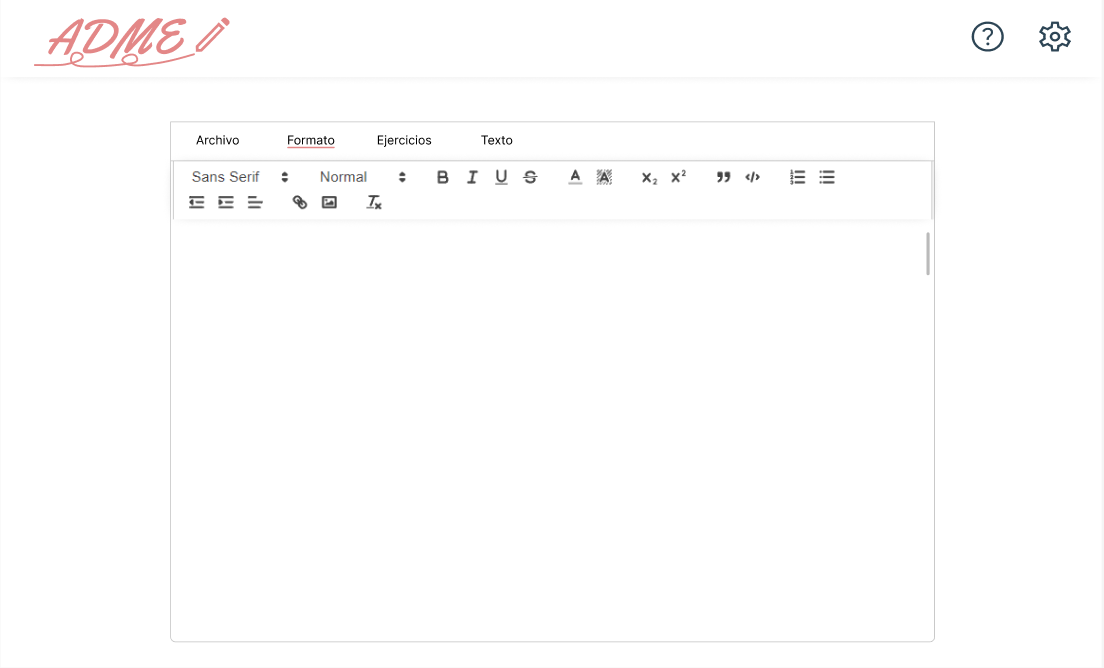
\includegraphics[width=15cm]{Diseño/Formato.PNG}
  \caption{Diseño de Formato pantalla de inicio.}
  \label{Forato}
\end{figure}

\begin{figure}[ht!]
  \centering
  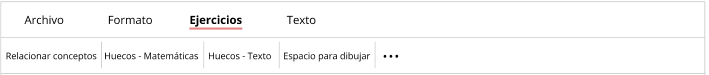
\includegraphics[width=15cm]{Diseño/Ejercicios.PNG}
  \caption{Diseño de Ejercicios pantalla de inicio.}
  \label{ejercicios}
\end{figure}

\begin{figure}[ht!]
  \centering
  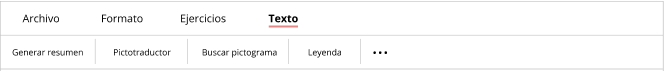
\includegraphics[width=15cm]{Diseño/Texto.PNG}
  \caption{Diseño de Texto pantalla de inicio.}
  \label{texto}
\end{figure}

\begin{figure}[ht!]
  \centering
  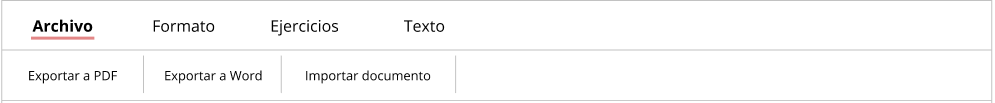
\includegraphics[width=15cm]{Diseño/Archivo.PNG}
  \caption{Diseño de Archivo pantalla de inicio.}
  \label{archivo}
\end{figure}

\subsubsection{Generar resumen}
El diseño de esta funcionalidad se muestra en la Figura \ref{resuemn} y se basa en el diseño de Álvaro Gómez, Figura \ref{fig:disenyoAlvaro03}. El usuario dispone de un panel en el que aparece el texto a resumir y el número de palabras que tendrá el resumen. Al pulsar el botón de resumir aparecerá en la parte inferior de la ventana modal una vista previa del resumen generado. El resultado de esta funcionalidad en el documento de trabajo se muestra en la Figura \ref{editable1}, en el ejercicio 3.

\begin{figure}[ht!]
  \centering
  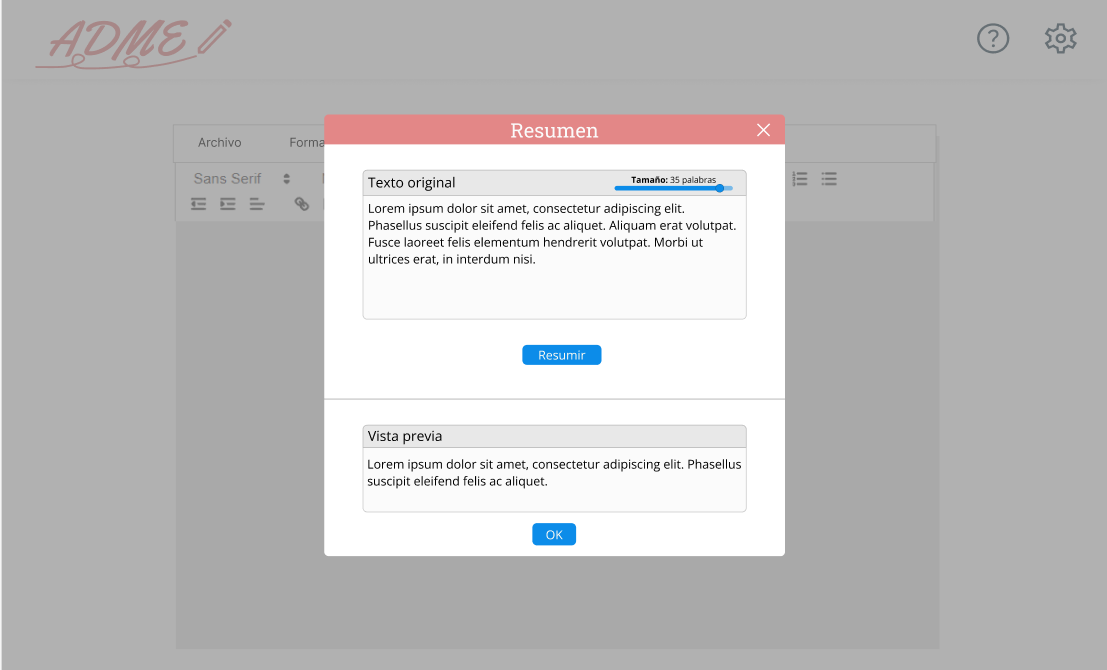
\includegraphics[width=15cm]{Diseño/Resumen.PNG}
  \caption{Diseño final de Generar resumen.}
  \label{resuemn}
\end{figure}

\subsubsection{Ejercicio de huecos}
El diseño de esta funcionalidad se muestra en la Figura \ref{definir_hueco}. Inicialmente habíamos pensado en que esta funcionalidad se pudiese hacer directamente sobre el documento de trabajo, pero al disponer de ventana modal y al ser complejo decidimos descartar dicha opción. En la ventana modal el usuario podrá escribir el texto. Una vez terminado le dará al botón de añadir huecos y pulsando sobre la palabra se pondrá un hueco y viceversa. Además, tiene la opción de elegir el tamaño de hueco, siendo pequeño (5 caracteres), mediano, que es el por defecto (12 caracteres) y el grande (23 caracteres). El resultado de esta funcionalidad en el documento de trabajo se muestra en la Figura \ref{editable3} en el ejercicio 3.

\begin{figure}[ht!]
  \centering
  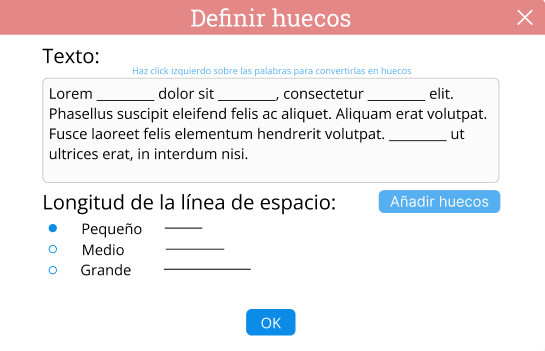
\includegraphics[width=0.7\textwidth]{Diseño/DefinirHuecos.PNG}
  \caption{Diseño final de Definir huecos.}
  \label{definir_hueco}
\end{figure}

\begin{figure}[ht!]
  \centering
  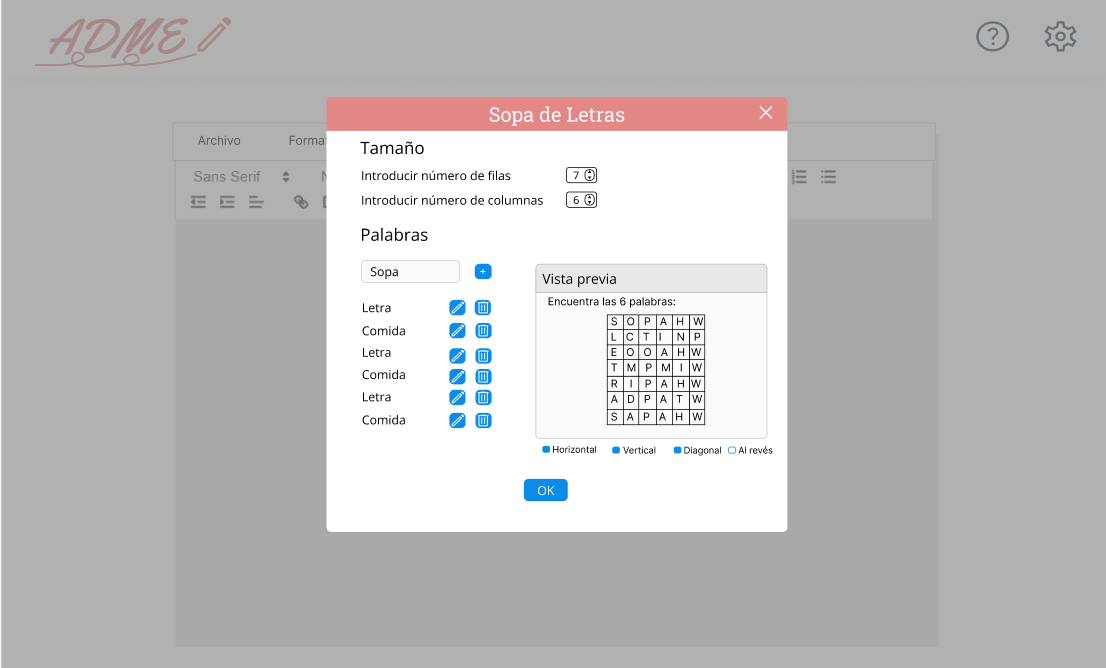
\includegraphics[width=0.7\textwidth]{Diseño/Sopa.PNG}
  \caption{Diseño final de la Sopa de letras.}
  \label{sopaLetras}
\end{figure}

\begin{figure}[ht!]
  \centering
  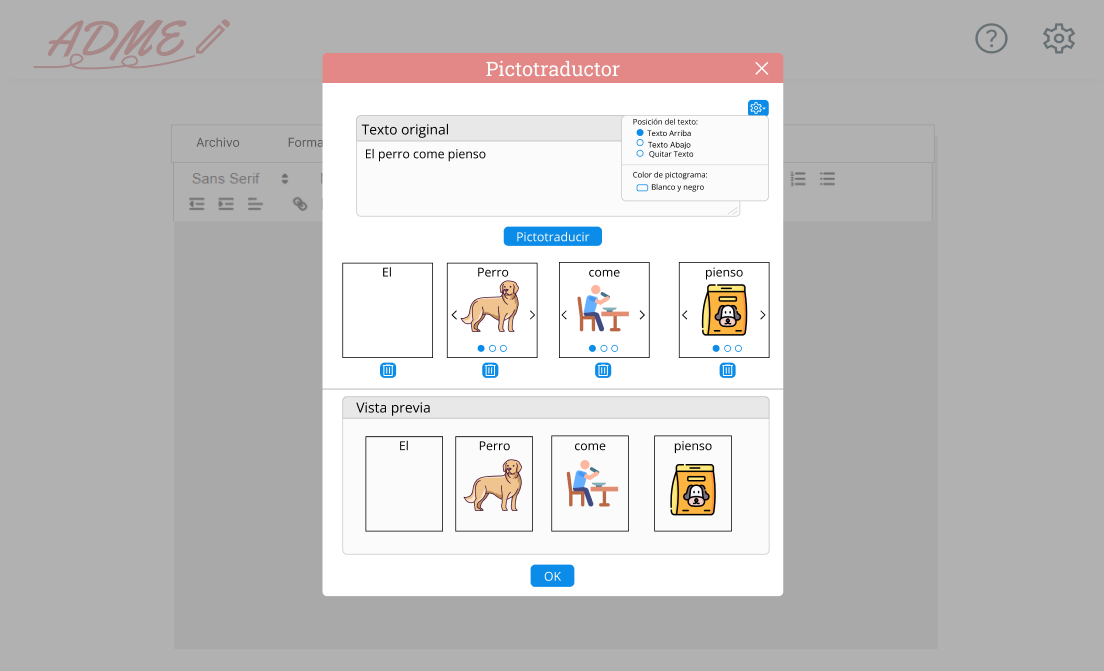
\includegraphics[width=0.7\textwidth]{Diseño/picto.PNG}
  \caption{Diseño final del pictotraductor.}
  \label{pictotraductor}
\end{figure}
\subsubsection{Sopa de letras}
El diseño de esta funcionalidad se muestra en la Figura \ref{sopaLetras} y se basa en el diseño de Alberto (Figura \ref{Alberto16}). Inicialmente pensamos en tener dos botones, uno para añadir nuevas palabras, que se iba moviendo a la vez que se creaba una nueva palabra, y otro que se encontraba al lado de cada palabra para eliminarla, pero llegamos a la conclusión
de que era mejor que el botón de añadir palabras fuera fijo y no cambiara de posición cada vez que se añadiese una nueva palabra ya que esto le aportaría comodidad y facilidad de uso. Para ayudar al usuario a que sea más intuitivo decidimos incluir dos campos para que el usuario introduzca las filas y las columnas de la sopa de letras. También añadimos otro campo donde poner la palabra y al darle al botón de añadir la palabra se pondrá debajo de dicho campo junto a dos botones, uno de edición y otro para eliminar la palabra. Además, añadimos varias opciones para que el usuario elija cómo disponer las palabras en la sopa de letras (horizontal, vertical, diagonal y al revés). El resultado de esta funcionalidad en el documento de trabajo se muestra en la Figura \ref{editable2} en el ejercicio 5.



\subsubsection{Pictotraductor}
El diseño de esta funcionalidad se muestra en la Figura \ref{pictotraductor} y se basa en el diseño de Johan (Figura \ref{Johan7}) y en la idea de Álvaro de que los pictogramas puedan cambiar en el caso de que haya varios pictogramas posibles para una misma palabra. Inicialmente se pensó un diseño bastante simple en el que había un campo para añadir un texto y al pulsar sobre el botón de traducir a pictogramas se mostrasen los pictogramas. Uno de los problemas que encontramos en este diseño fue la falta de consideración de diversas opciones necesarias para satisfacer las necesidades del usuario en cuanto al diseño de los pictogramas. Estas opciones incluyen el posicionamiento y existencia del texto en relación al pictograma, así como la posibilidad de personalizar el color del mismo. Finalmente mantuvimos el campo de añadir el texto a traducir y el botón que te muestra los pictogramas con su respectiva palabra y añadimos un desplegable para escoger las opciones de posicionamiento de la palabra a la que se refiere el pictograma, color del pictograma y quitar la palabra asociada al pictograma. Por otra parte, cada pictograma tiene su propio botón de eliminar y unas flechas que permiten seleccionar otro de los pictogramas disponibles para la misma palabra del pictograma, en el caso de que haya varias opciones. El resultado de esta funcionalidad en el documento de trabajo se muestra en la Figura \ref{editable1} en el ejercicio 3.

\begin{figure}[ht!]
  \centering
  \includegraphics[width=0.55\textwidth]{Diseño/Flechas.PNG}
  \caption{Diseño final de ejercicios de fechas.}
  \label{flechas}
\end{figure}

\subsubsection{Ejercicio de flechas}
El diseño de esta funcionalidad se muestra en la Figura \ref{flechas} y se basa en el diseño de Dunia Namour (Figura \ref{dunia4}). Inicialmente dábamos la opción de solo hacer dos columnas para relacionar con flechas, pero nos dimos cuenta de que el usuario debería poder elegir tantas columnas como desee. Tampoco tuvimos en cuenta que el usuario podría querer desordenar las columnas para que no tenga que pensar en el orden de las palabras. Con todo lo anterior creamos una ventana modal en la que se debe introducir el número filas y columnas, lo que genera tantas columnas vacías como haya indicado el usuario. Una vez que el usuario rellena dichas columnas tiene la opción de reordenar, la cual reordenaría cada columna. La ventana modal dispone de una vista previa en la cual se mostrará cómo quedaría el ejercicio de flechas, generándose automáticamente cada vez que el usuario realice un cambio en alguna de las columnas. El resultado de esta funcionalidad en el documento de trabajo se muestra en la Figura \ref{editable1} en el ejercicio 1.


\subsubsection{Ejercicio de desarrollo}
Partimos del diseño de AdaptaMaterialEscolar 1.0. Dicho diseño no permitía al usuario cambiar el tipo de pauta ni elegir el interlineado. Todo lo mencionado anteriormente se ha añadido al nuevo diseño y también se ha incluido una vista previa que se genera automáticamente cada vez que se haga un cambio para que el usuario pueda visualizar cómo quedará el ejercicio. El diseño de esta funcionalidad se muestra en la Figura \ref{DesarrolloFinal}. El resultado de esta funcionalidad en el documento de trabajo se muestra en la Figura \ref{editable1} en el ejercicio 2.

\begin{figure}[ht!]
  \centering
  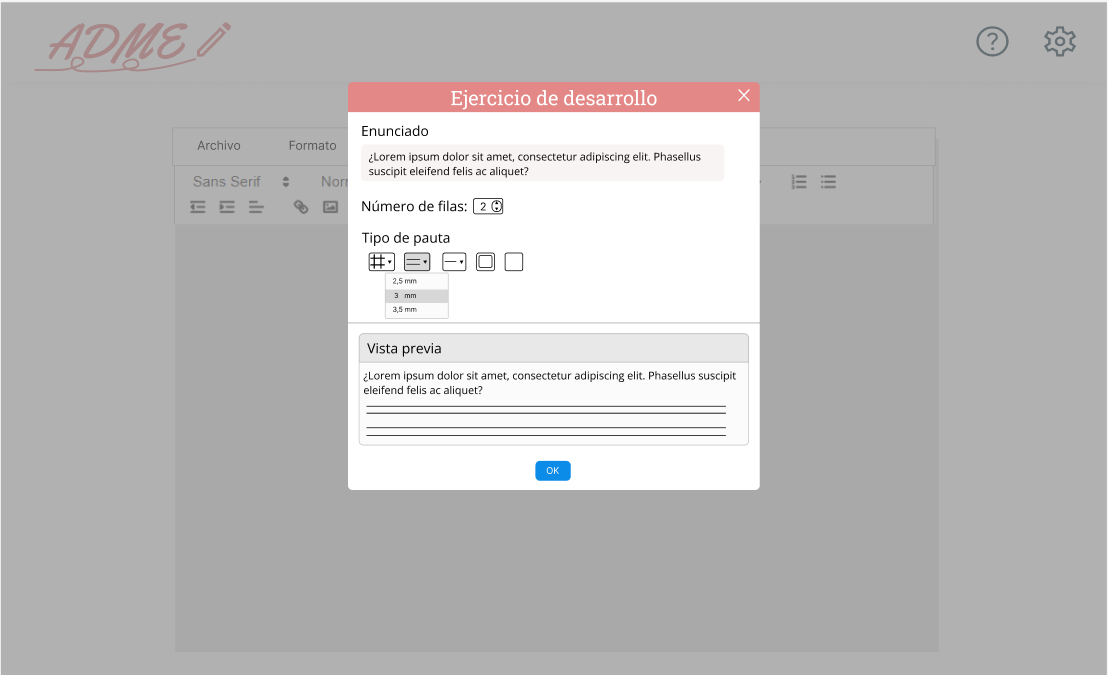
\includegraphics[width=0.7\textwidth]{Diseño/Desarollo.PNG}
  \caption{Diseño final de ejercicios de desarrollar.}
  \label{DesarrolloFinal}
\end{figure}

\begin{figure}[ht!]
  \centering
  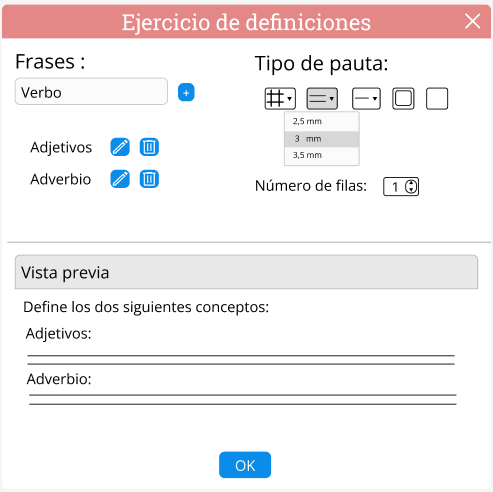
\includegraphics[width=0.7\textwidth]{Diseño/definiciones.PNG}
  \caption{Diseño final de ejercicios de definiciones.}
  \label{defi}
\end{figure}

\subsubsection{Ejercicio de definiciones}
Partimos del diseño de AdaptaMaterialEscolar 1.0. Dicho diseño tenía los mismos problemas que el de ejercicios de desarrollo. El diseño final de esta funcionalidad se muestra en la Figura \ref{defi}. El resultado de esta funcionalidad en el documento de trabajo se muestra en la Figura \ref{editable2} en el ejercicio 3.


\subsubsection{Ejercicios de espacio para dibujar}
El diseño de esta funcionalidad se muestra en la Figura \ref{espaciosDibu}. En esta funcionalidad el usuario inicialmente tendrá que escribir el enunciado e indicar el espacio que desea dejar para dibujar. Además, incorpora una opción de recuadrar que hace un recuadro del tamaño indicado. El resultado de esta funcionalidad en el documento de trabajo se muestra en la Figura \ref{editable3} en el ejercicio 5.


\subsubsection{Leyenda de colores}
El diseño final de esta funcionalidad se muestra en la Figura \ref{LeyendaColores} y para realizar esta funcionalidad no hemos basado en el diseño de todos los integrantes ya que son bastante parecidos. También hemos utilizado como referencia la funcionalidad de definir conceptos. En este caso cuando se añade un nuevo concepto también se ha de escoger un color para cada palabra. Además, se ha de incluir un título para la leyenda. La leyenda de color se situará en el documento de trabajo donde se encuentre el cursor y el usuario podrá ajustar su posicionamiento. El resultado de esta funcionalidad en el documento de trabajo se muestra en la Figura \ref{editable2} en el ejercicio 2.

\begin{multicols}{2}
  \begin{figure}[H]
    \centering
    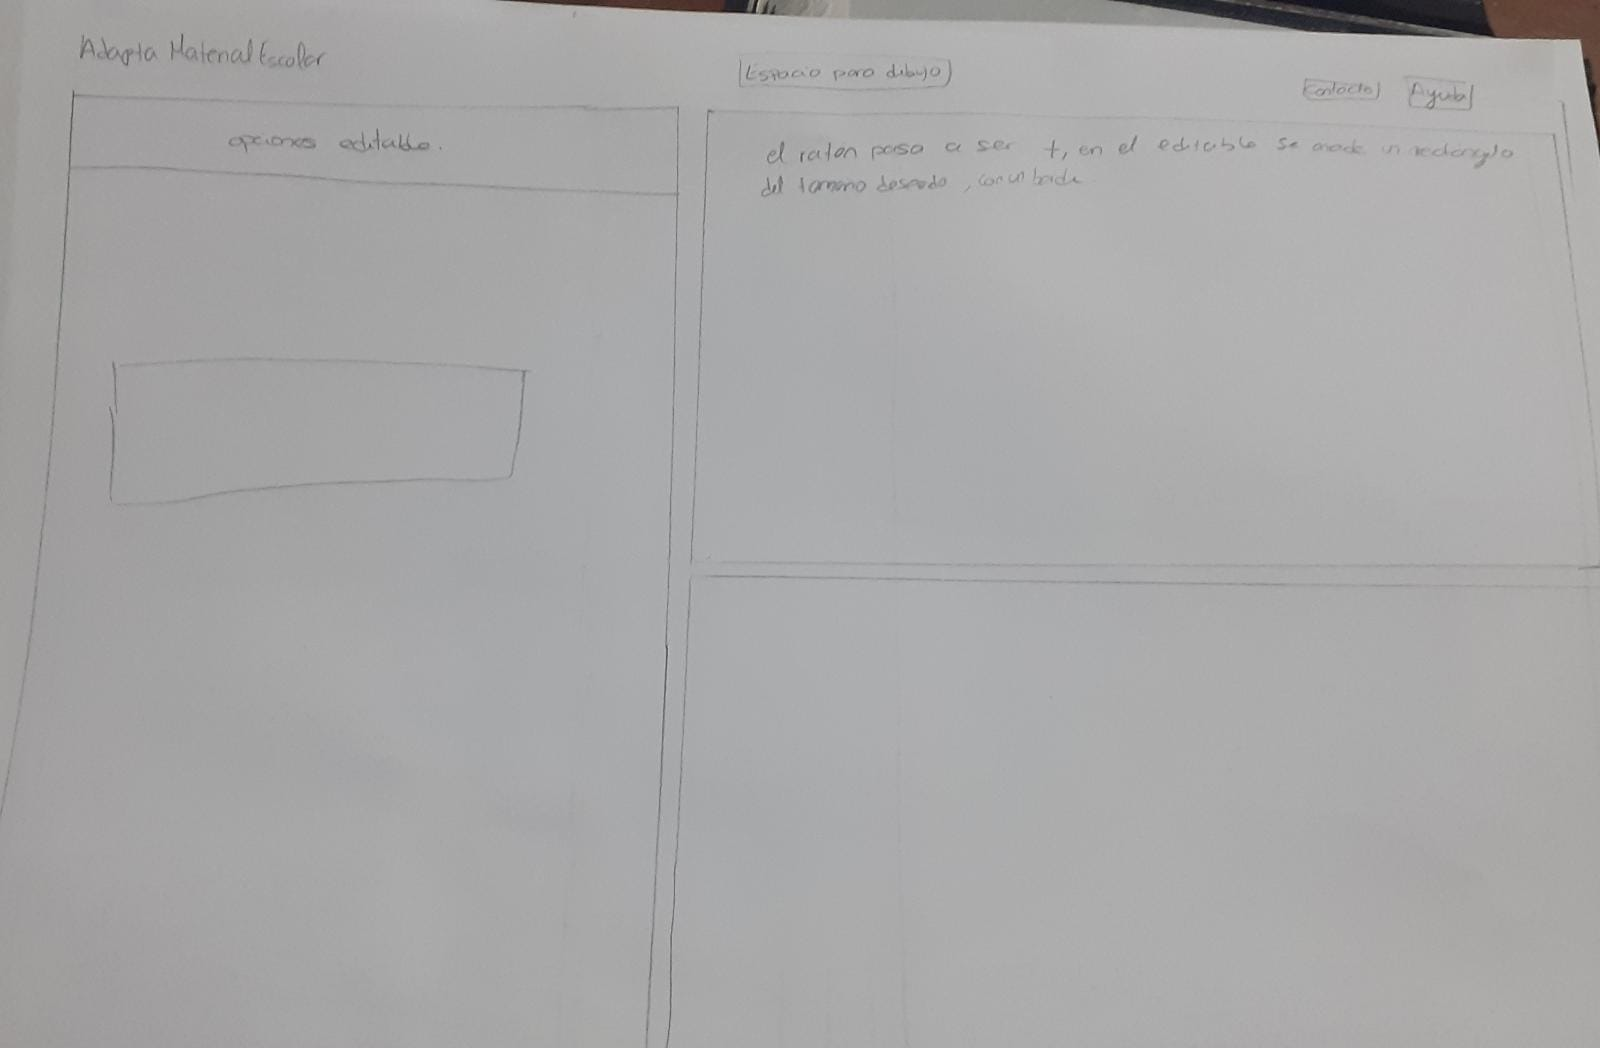
\includegraphics[width=0.5\textwidth]{Diseño/espacioDibu.PNG}
    \caption{Diseño final ejercicios espacios para dibujar.}
    \label{espaciosDibu}
  \end{figure}
  \begin{figure}[H]
    \centering
    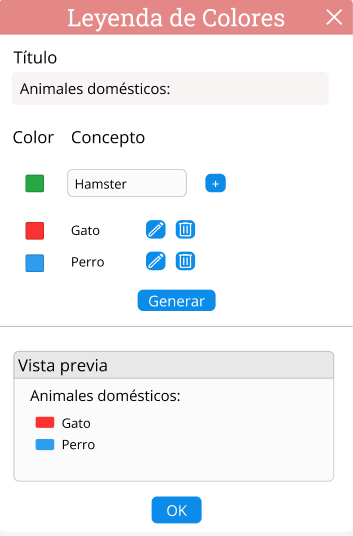
\includegraphics[width=0.4\textwidth]{Diseño/Leyenda.PNG}
    \caption{Diseño final leyenda de colores.}
    \label{LeyendaColores}
  \end{figure}
\end{multicols}

\subsubsection{Ejercicio de matemáticas con huecos}
El diseño de esta funcionalidad se muestra en la Figura \ref{matesHueco} y para realizarla nos hemos basado en el diseño de Dunia Namour, (Figura \ref{dunia6}) y en la idea de Johan Salvatierra de que al pulsar la tecla \textit{espacio} se genere un hueco. Para introducir huecos en una fórmula matemática el usuario tendrá que darle a la barra espaciadora. Cuando termine de escribir la fórmula al darle al botón de \textit{OK} se introducirá en el documento de trabajo con un cuadrado vacío en cada hueco. El resultado de esta funcionalidad en el documento de trabajo se muestra en la Figura \ref{editable3} en el ejercicio 2.

\begin{figure}[ht!]
  \centering
  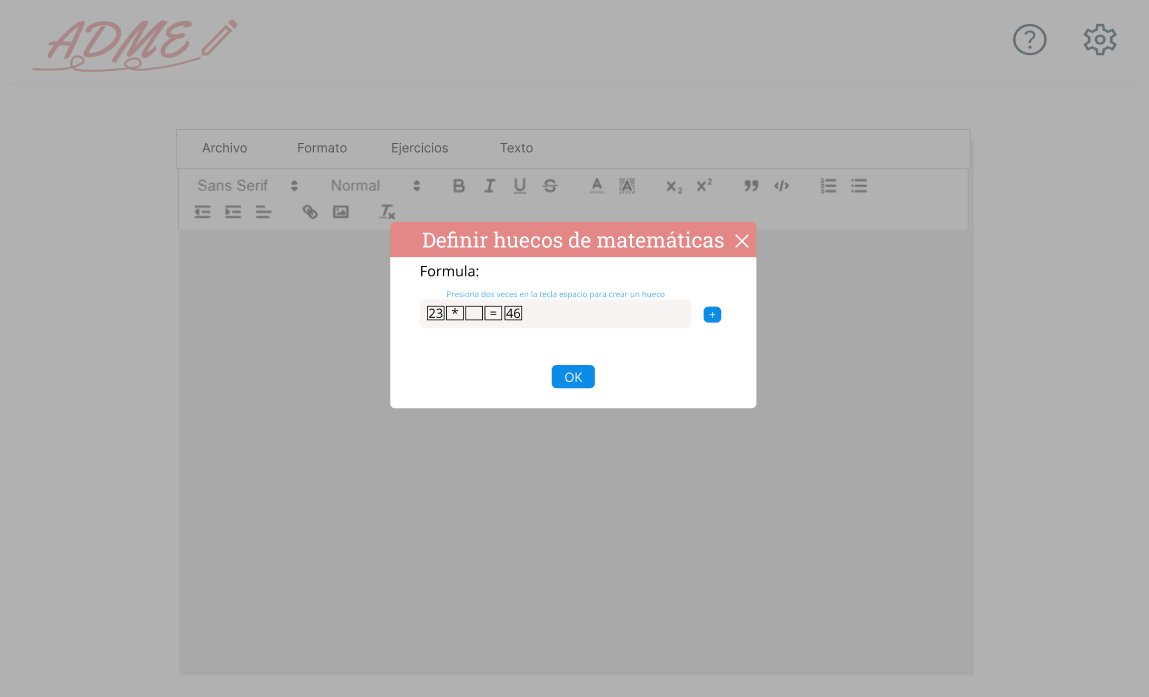
\includegraphics[width=0.7\textwidth]{Diseño/EjerMatesHuecos.PNG}
  \caption{Diseño final ejercicios de matemáticas con huecos.}
  \label{matesHueco}
\end{figure}
\begin{figure}[ht!]
  \centering
  \includegraphics[width=15cm]{Diseño/configuracion.PNG}
  \caption{Diseño final de la configuración general.}
  \label{configu}
\end{figure}
\subsubsection{Configuración general}
Debido a que gran parte de las funcionalidades tienen varias opciones hemos decidido crear una página de configuración para poder definir los ajustes por defecto. En esta página hay una configuración general por cada tipo de funcionalidad. El diseño de la configuración se muestra en la Figura \ref{configu}. Esta página surgió durante el \textit{brainstorming} con las tutoras por la necesidad de tener ajustes por defecto.



\begin{figure}[ht!]
  \centering
  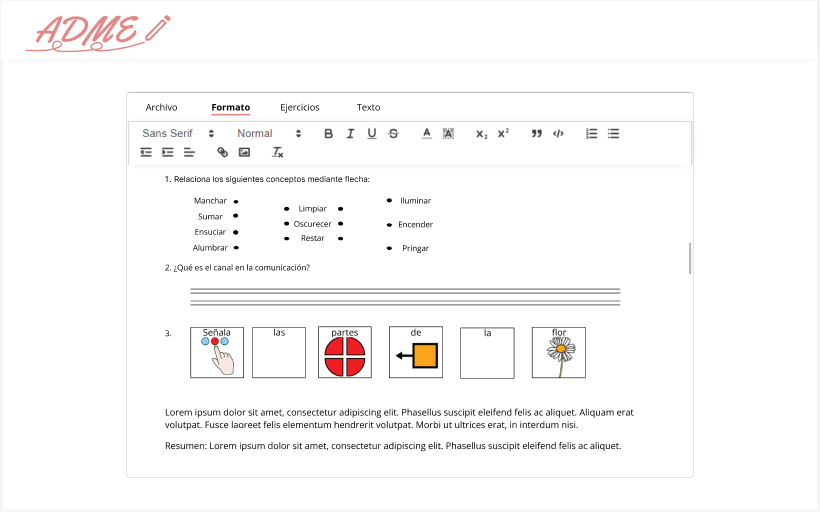
\includegraphics[width=15cm]{Diseño/Editable1.PNG}
  \caption{Resultado de las funcionalidades en el documento de trabajo.}
  \label{editable1}
\end{figure}

\begin{figure}[ht!]
  \centering
  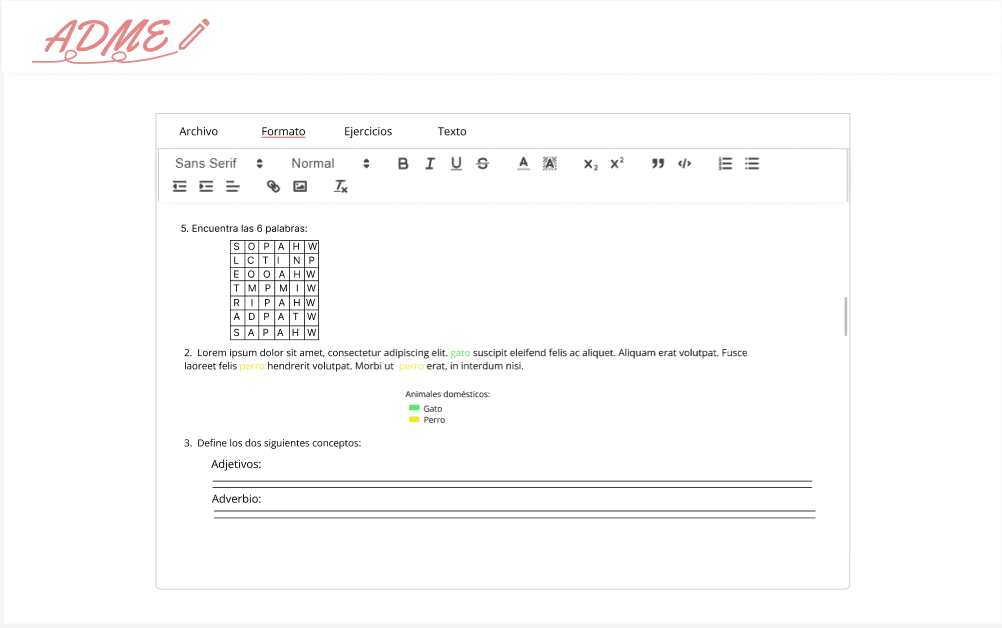
\includegraphics[width=15cm]{Diseño/editable2.PNG}
  \caption{Resultado de las funcionalidades en el documento de trabajo.}
  \label{editable2}
\end{figure}

\begin{figure}[ht!]
  \centering
  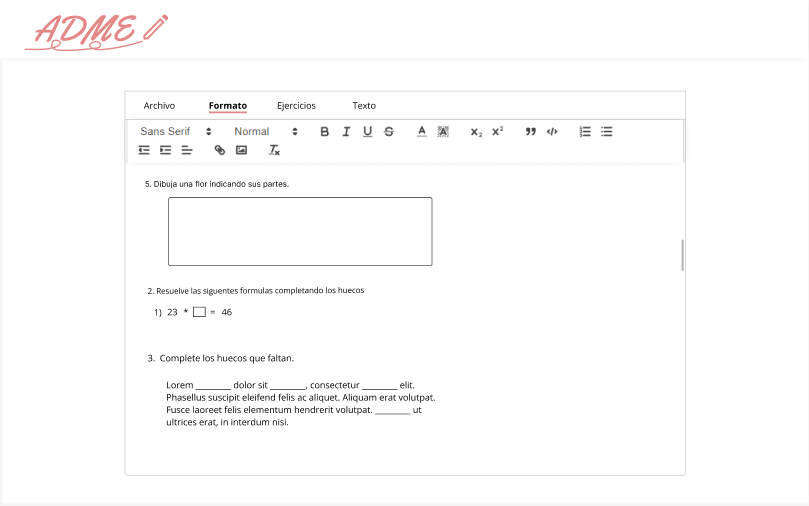
\includegraphics[width=15cm]{Diseño/Editable3.PNG}
  \caption{Resultado de las funcionalidades en el documento de trabajo.}
  \label{editable3}
\end{figure}

\section{Implementación}
\label{sec:implmentaction}
AdaptaMaterialEscolar es una aplicación web implementada con React y el código se encuentra en el repositorio del grupo NIL en GitHub\footnote{\url{https://github.com/NILGroup/TFG-22-23-AdaptaMaterialEscolar2.0/tree/master/Codigo}}.

En las siguientes secciones se explicará en detalle la arquitectura y cómo se han implementado cada una de las funcionalidades de la aplicación.
\subsection{Arquitectura}
\label{sub:Arquitectura}
Desde el punto de vista de la arquitectura, se han mantenido partes de AdaptaMaterialEscolar 1.0 (ver Sección \ref{cap:adaptaMaterial}) y se han realizado ciertas modificaciones.

En primer lugar, se ha decidido mantener React debido a la escalabilidad que proporciona y a que es una de las bibliotecas más utilizadas\footnote{\url{https://gist.github.com/tkrotoff/b1caa4c3a185629299ec234d2314e190}} sin embargo, al haber pasado 2 años del TFG de AdaptaMaterialEscolar 1.0 se han producido una serie de actualizaciones con respecto a esta biblioteca. Uno de los principales cambios en la arquitectura de la aplicación ha sido la transición de los componentes basados en clases a los componentes funcionales. Otra actualización importante que se ha llevado a cabo en AdaptaMaterialEscolar 2.0 es la actualización del router de React a la última versión disponible, ya que dicha actualización  permite aprovechar las últimas funcionalidades y mejoras introducidas en esta librería.

En cuanto a las APIs y bibliotecas hemos empleado la API de ARASAAC y la biblioteca de \textit{word-search} ya utilizadas por AdaptaMaterialEscolar 1.0.

En cuanto a las modificaciones con respecto a la aplicación incial, se decidió llevar a cabo una refactorización en la arquitectura del proyecto. En concreto se modificó la estructura \textit{serverless} por una arquitectura basada en un servidor \textit{backend} que hace de intermediario entre el cliente y las APIs. Este cambio se ha llevado a cabo porque actualmente los navegadores utilizan el mecanismo \textit{CORS}, es una política de  seguridad que impide que una página web cargada desde un dominio A pueda realizar solicitudes a recursos alojados en un dominio B sin que este último lo haya permitido previamente. Esto implica que no se pueden consumir APIs por parte del cliente a menos que la API haya desactivado dicho mecanismo.

En relación a Redux, lo descartamos ya que la comunicación entre los componentes es descendente, es decir, los datos y el estado son transmitidos desde un componente padre a sus componentes hijos. En este contexto, Redux no ofrecía una ventaja significativa en términos de gestión del estado de los componentes, ya que la cantidad de datos a manejar era relativamente pequeña y no se requería una gestión centralizada de los mismos.

Por otra parte, se decidió cambiar el editor, ya que la licencia de CKEditor 4.0 que se adquirió para AdaptaMaterialEscolar 1.0 expiró y ya no ofrecen licencias académicas para la versión más actualizada, CKEditor 5.0. Se decidió utilizar Slate como editor, como se explicará con mayor detalle en la Sección \ref{Editor}. Se trata de un editor basado en componentes reutilizables que se integra facilmente con React. En la Figura \ref{fig:arquitecturageneral} se muestra una visión general de la arquitectura general de AdaptaMaterialEscolar 2.0.

Tanto React como Slate se apoyan en el patrón \textit{Composite}\footnote{\url{https://refactoring.guru/es/design-patterns/composite}} el cual permite generar un componente complejo mediante la anidación de componentes simples. Por otro lado, también hemos usado el patrón creacional \textit{Factory}\footnote{\url{https://refactoring.guru/es/design-patterns/factory-method}} que nos permite crear objetos sin tener que conocer los detalles de su creación. Lo hemos usado para la creación de los modales y de las distintas barras de herramientas que se encuentran en el editor. En la Figura \ref{fig:diagramaComponentes} se muestra el diagrama de componentes de nuestra aplicación.
\begin{figure}[ht!]
  \centering
  \begin{subfigure}{\textwidth}
    \centering
    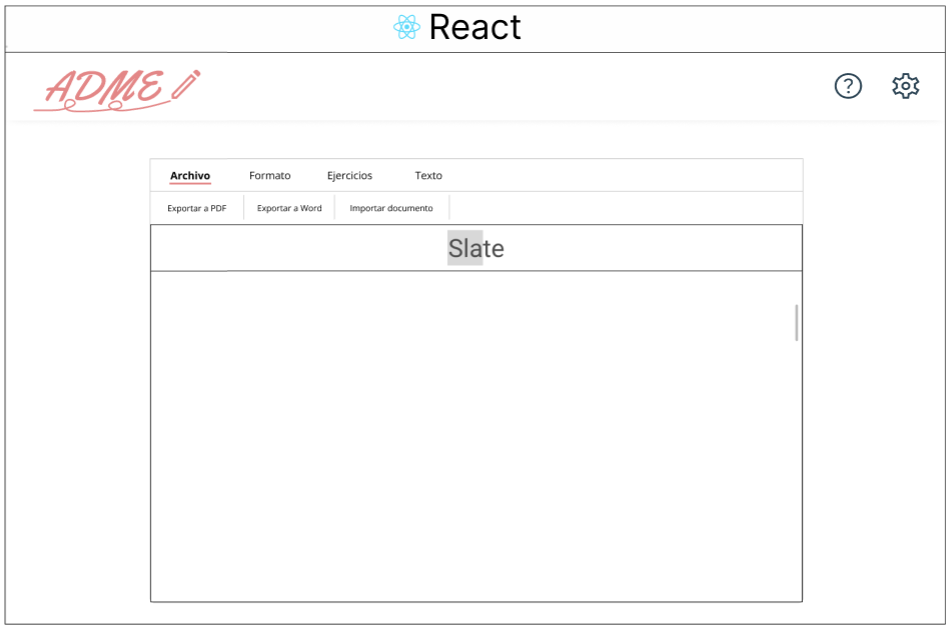
\includegraphics[width=0.7\textwidth]{Arquitectura/ArquitecturaPaginaInicio.png}
    \caption{Visión general de la página de inicio}
    \label{fig:arquitecturageneral1}
  \end{subfigure}

  \begin{subfigure}{\textwidth}
    \centering
    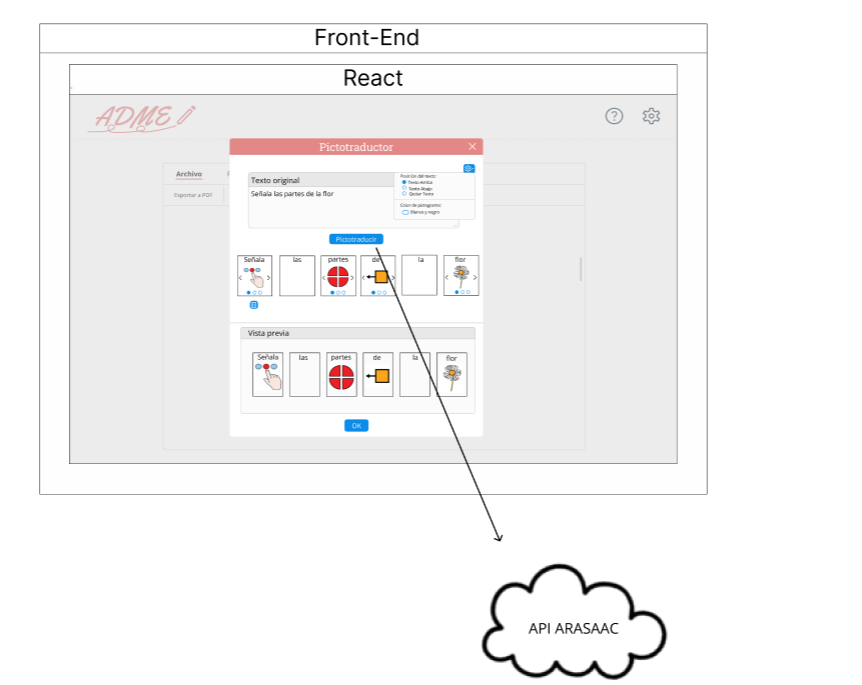
\includegraphics[width=0.7\textwidth]{Arquitectura/ArquitecturaPictoTraductor.png}
    \caption{Visión general de funcionalidad con conexión a API}
    \label{fig:arquitecturageneral2}
  \end{subfigure}
  \caption{Visión general de AdaptaMaterialEscolar 2.0}
  \label{fig:arquitecturageneral}
\end{figure}

\begin{figure}[ht!]
  \centering
  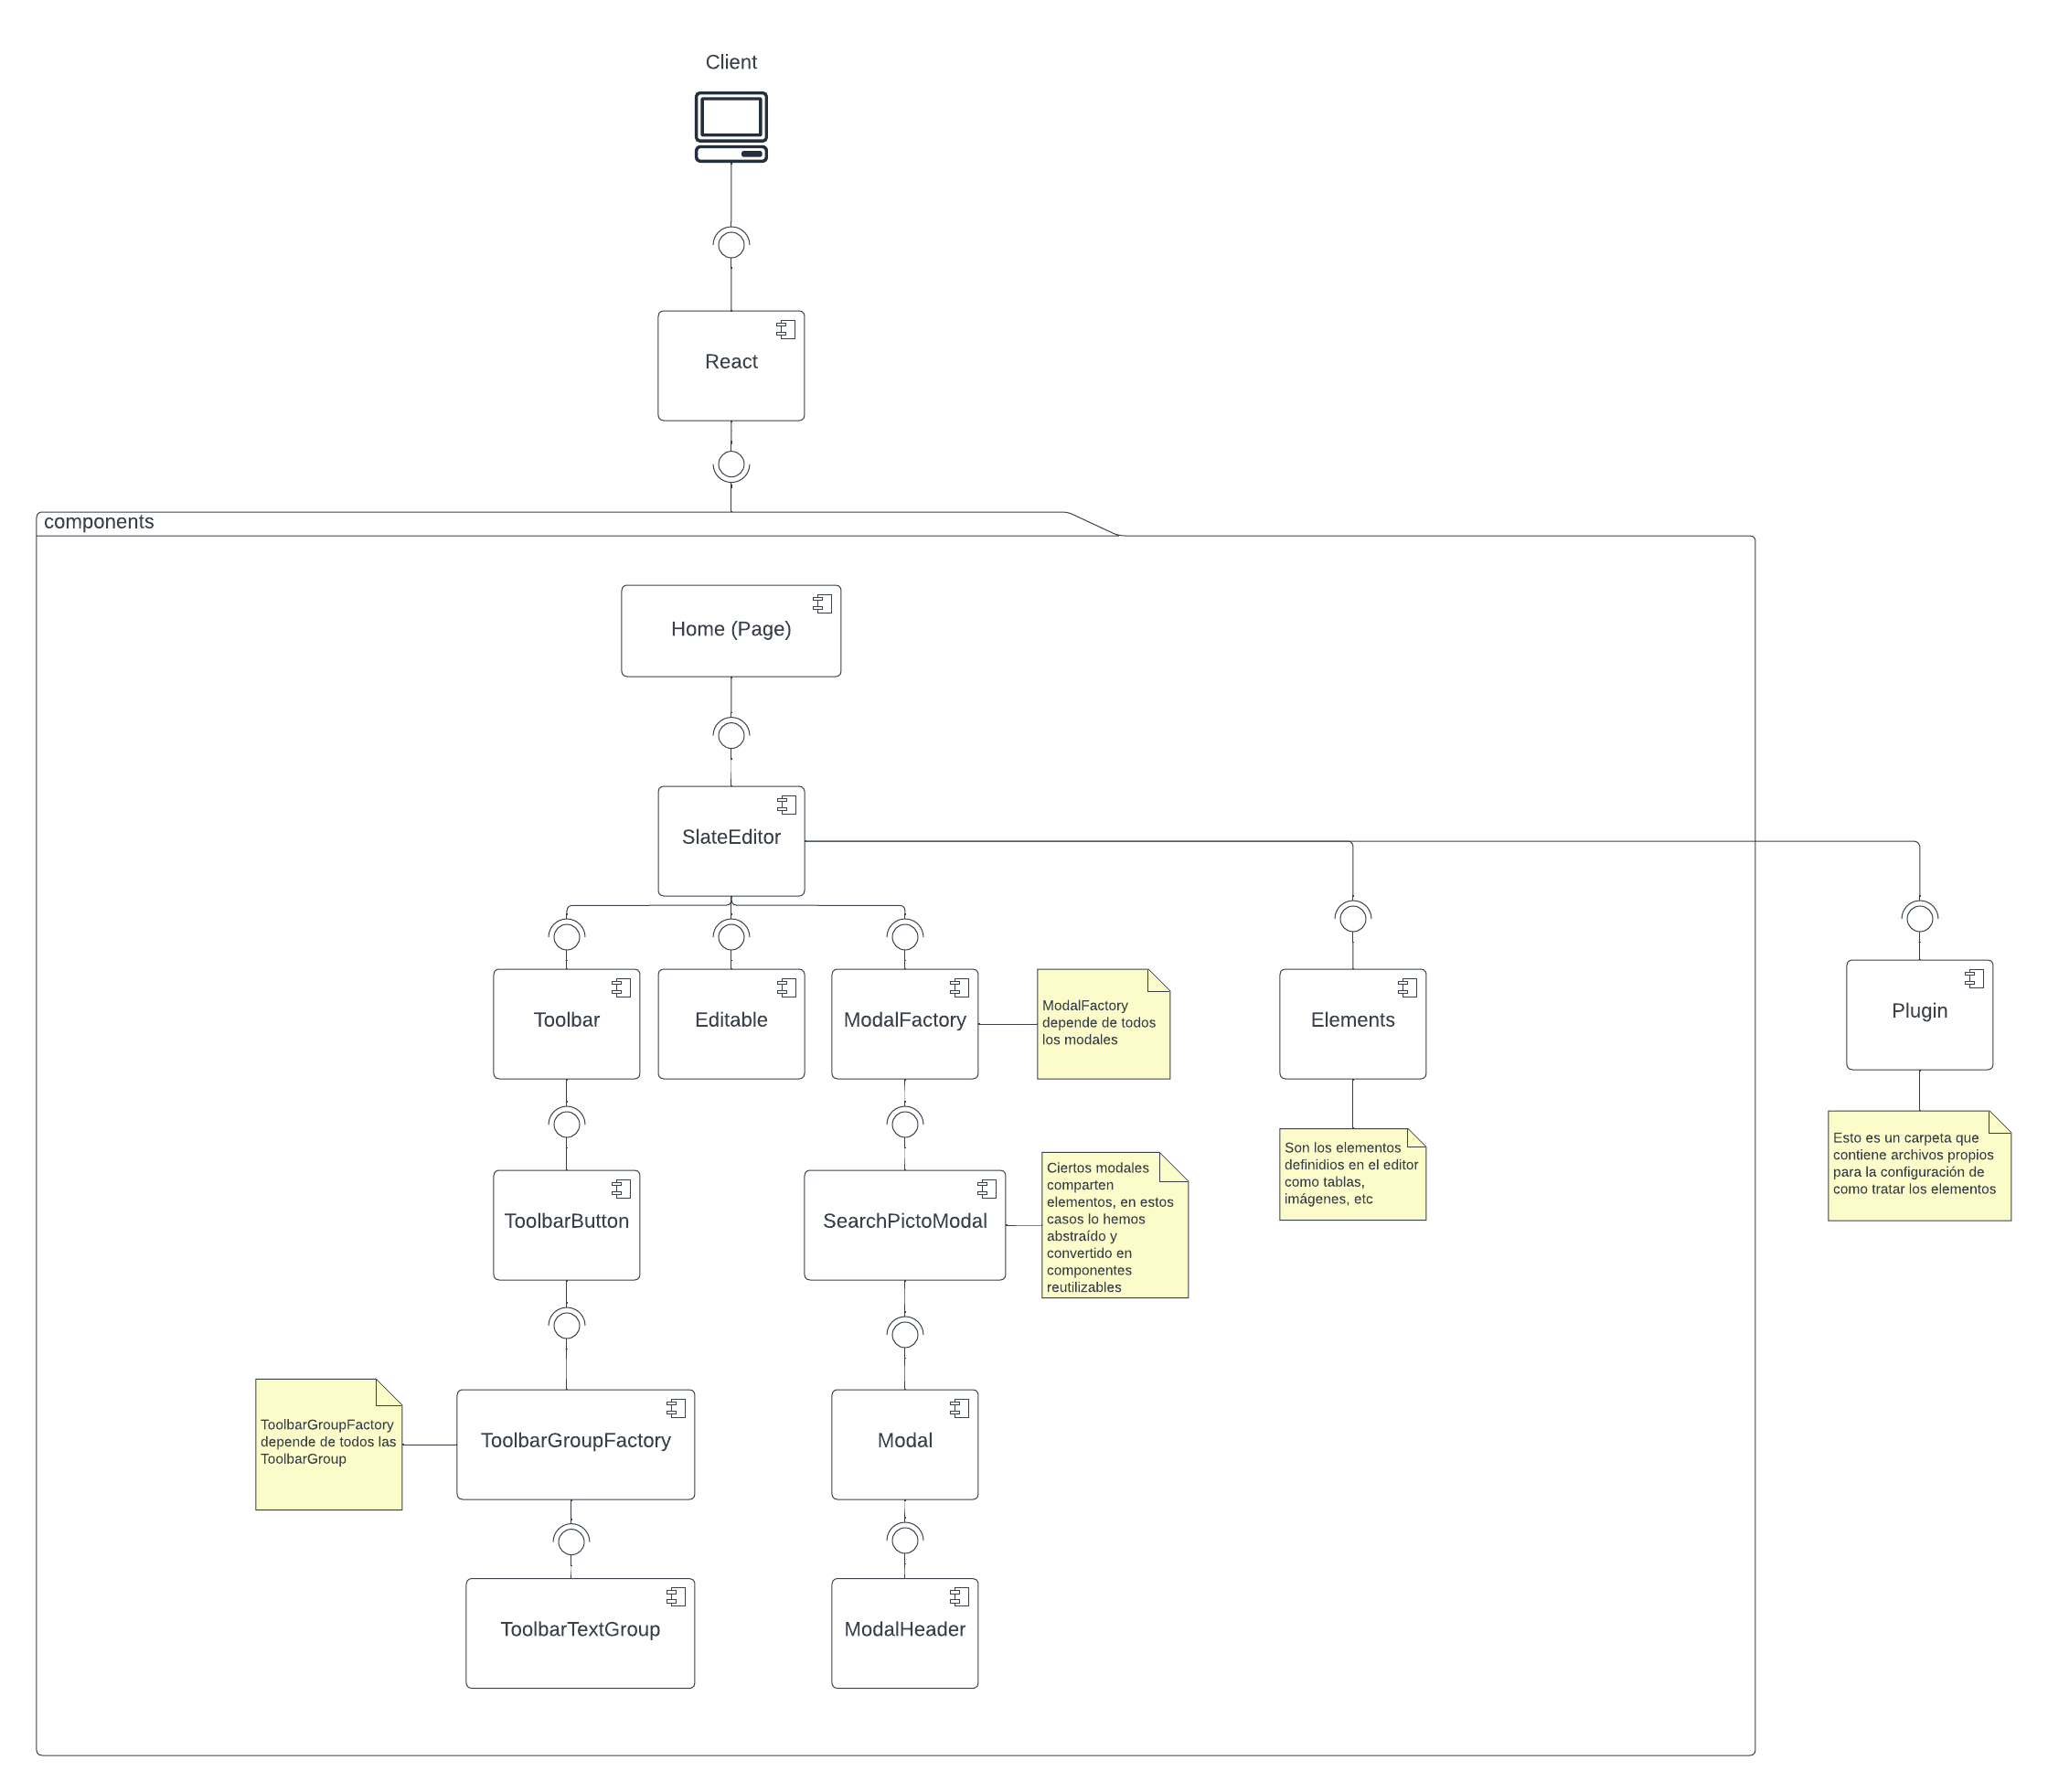
\includegraphics[width=0.8\textwidth]{Arquitectura/Diagrama_de_Componentes.png}
  \caption{Diagrama de componentes de AdaptaMaterialEscolar 2.0}
  \label{fig:diagramaComponentes}
\end{figure}

\subsection{Editor}
\label{Editor}
El editor de texto que hemos empleado es Slate (explicado en la Sección \ref{sec:Slate}). En esta sección, se describirá en detalle la estructura del editor y su integración en nuestra aplicación de adaptación curricular.

\subsubsection{Estructura del editor}
El editor consta de tres partes: barra de selección de barra de herramientas, barra de herramientas seleccionada y la zona de escritura. Como se ve en la Figura \ref{Forato} la barra de selección de herramientas dispone de los siguientes elementos: Archivo, Formato, Ejercicios y Texto. Estos elementos han sido ya explicados en la Sección \ref{cap:requisitos}, y cabe destacar que hemos empleado el patrón \textit{Factory} para separar la creación del elemento del creador. De esta forma se logra una mayor escalabilidad.
A continuación se explicará en detalle cada una de las barras de herramientas disponibles en el editor:

\begin{itemize}
  \item Archivo: Esta barra contiene las opciones relacionadas con el manejo de archivos, que son:
        \begin{itemize}
          \item  Exportar a PDF: Permite exportar a un documento en formato \textit{.pdf}. Esto es posible gracias a un plugin que serializa el contenido permitiendo que sea transferible a otro formato.
          \item  Exportar a Word: Permite exportar a un documento en formato \textit{.docx}, y emplea el mismo sistema que el exportar a PDF.
          \item Importar documento: A partir de un documento con extensión \textit{.docx} extrae el contenido, lo serializa mediante un plugin y se transfiere al editor.
        \end{itemize}
  \item Formato: Esta barra contiene opciones para formatear el texto que se está editando. Las opciones que incluye son:
        \begin{itemize}
          \item Negrita: Permite cambiar el formato de texto a negrita.
          \item Tabla: Permite crear una tabla del numero de filas y columnas elegidas por el usuario con un maximo de 6 filas por 6 columnas.
        \end{itemize}
  \item Ejercicios: Esta barra dispone de varias opciones para crear ejercicios:
        \begin{itemize}
          \item Completar huecos: Esta opción despliega un modal que permite introducir la información necesaria para crear un ejercicio de completar huecos. Una vez creado el ejercicio, desde el padre de la estructura interna del editor, este se introduce en un nodo parrafo.
          \item Sopa de letras: Si se selecciona esta opción, se abrirá un modal que al usuario permitirá introducir la información requerida para crear un ejercicio de sopa de letras. La sopa de letras que se crea se introduce en un nodo que tiene dos hijos: el primero es un nodo de tipo párrafo y el segundo es un nodo de tipo tabla.
          \item Definiciones: Al hacer clic en esta opción, aparecerá un modal que al usuario permitirá introducir la información necesaria para crear un ejercicio de definiciones. Para introducir el ejercicio en el documento base del editor, se define un nodo llamado ``definition'' que encapsula el nodo párrafo para el enunciado, otro nodo párrafo por cada concepto y un nodo denominado ``staff'' para los tipos de pauta.
          \item Verdadero/Falso: Esta opción activa un modal donde puede insertar la información necesaria para definir el ejercicio de verdadero o falso. Para guardar este ejercicio en el editor se define un nodo denominado ``list'' que contine un nodo párrafo para el enunciado y tantos nodos párrafo como conceptos introduzca el usuario. En el cual se encuentra un nodo llamado ``icon'' para el cuadrado donde el alumno indicara si es verdadero o falso.
          \item Desarrollo: Esta opción despliega un modal que permite introducir la información necesaria para crear un ejercicio de desarrollo, y emplea el nodo ``definition'' este es igual que el nodo ``definition'' pero como si tuviera un solo concepto.
          \item Formula Matemática: Esta función, desde el punto de vista del editor, es igual a la de completar huecos.
        \end{itemize}
  \item Texto: Esta barra de herramientas contiene opciones para manipular el texto. Todas, al igual que la anterior barra de herramientas, despliegan un modal para obtener la información necesaria para crear el nodo:
        \begin{itemize}
          \item Generar resumen: Con la información obtenida se crea un nodo de tipo párrafo.
          \item Picotraductor: Esta función obtiene una imagen usando la API de ARASAAC que se introduce en un nodo que hemos denominado ``image''.
        \end{itemize}
\end{itemize}

Cabe mencionar que las opciones en las barras de herramientas de Ejercicios y Texto generan un modal y estos modales también son gestionados con el patrón \textit{Factory} como se explicó en la Sección \ref{sub:Arquitectura}. Además los nodos de estas barras se introducen en el editor a través de la función ``insertNodes'' que proporciona Slate.


\subsubsection{Integración del editor con la aplicación}
Para integrar Slate en nuestra aplicación hemos empleado React-Slate, una librería React para crear editores de texto basada en Slate. Su configuración inicial solo proporciona la funcionalidad de escribir y borrar por lo que el resto de funcionalidades deben ser añadidas incluyendo las funciones de un editor común. Esta librería proporciona el componente ``Editable'' que es como una especie de lienzo,  el componente ``Slate'' que es el marco de este lienzo y ``withReact'' que es un envoltorio de Slate que permite integrar de forma fácil y eficiente la biblioteca de edición de texto con React, es decir, permite que el editor se actualice en tiempo real.

Hemos creado varios tipos de nodos en nuestro proyecto, incluyendo nodos hoja, nodos inline, nodos de bloque y nodos elemento. Estos tipos de nodos se describen en la sección \ref{sec:Slate}.

Para los nodos hoja, hemos creado varios tipos, entre ellos:

\begin{itemize}
  \item Nodo negrita: Implementado con la etiqueta ``strong'' de HTML.
  \item Nodo itálica: Implementado con la etiqueta ``em'' de HTML.
  \item Nodo subrayado: Implementado con la etiqueta ``u'' de HTML.
  \item Nodo tachado: Implementado con la etiqueta ``s'' de HTML.
  \item Nodo de texto estilado: Implementado con la etiqueta ``span'' y un estilo dinámico que permite al usuario cambiar el estilo mediante un botón. El estilo puede incluir cambios de fuente, tamaño, color de texto y color de fondo.
\end{itemize}
Para implementar estos nodos hoja, hemos utilizado la función ``addMark'' de Slate, que añade el nodo hoja al valor seleccionado.

Para los nodos de bloque, hemos creado los siguientes tipos:

\begin{itemize}
  \item Nodo lista ordenada: Implementado con la etiqueta ``ol'' de HTML.
  \item Nodo lista desordenada: Implementado con la etiqueta ``ul'' de HTML.
  \item Nodo elemento de lista: Implementado con la etiqueta ``li'' de HTML.
\end{itemize}

Es importante mencionar que para los nodos de bloque es necesario cambiar el nodo actual, que es un párrafo, por el nodo de bloque elegido. Esto se logra utilizando la función ``setNodes'' de Slate. Además, para los nodos lista ordenada y lista desordenada, hemos utilizado la función ``wrapNodes'', que permite envolver los nodos elegidos. Esto se debe a que las etiquetas ``ol'' y ``ul'' tienen una estructura de envoltura y deben envolver los nodos elemento de lista.

Los nodos inline son similares a los nodos de bloque, pero no ocupan todo el párrafo, lo que permite agregar texto o cualquier otra cosa después de ellos. Por defecto, Slate trata los nuevos nodos como nodos de bloque, por lo que es necesario reescribir este comportamiento. Lo hacemos mediante plugins, que son funciones que reescriben el comportamiento del editor y devuelven el editor con las funciones redefinidas. El plugin que permite definir los nodos inline se llama ``withInline''. Esta función detecta qué nodos son inline y añade los nodos que consideramos necesarios, como ``imagen'' e ``icono''.
\begin{itemize}
  \item Nodo imagen: Su estructura se basa en la etiqueta ``img'' de HTML, la cual recibe una URL a través de sus propiedades. Para que este nodo reaccione cuando el cursor está encima de él, hemos utilizado las funciones ``useSelected'' y ``useFocused'' de Slate. La primera devuelve ``true'' si el nodo está seleccionado, y la segunda devuelve ``true'' si el cursor está en el nodo. Por otro parte, este nodo tuve ciertos problemas debido a que slate considera de partida que todos los nodos son editables para esto supone que el nodo esta forma por una serie de unidades. Esto produce una serie de problemas a la hora de borrar y seleccionar porque no encuentra la forma de tratarlo. Para esto lo que hicimos es que se comportaran en si como una unidad esto se logra mediante un plugin denominada ``withEmbeds'' este hace que cuando se detecta este nodo diga que esta vacio por
        propiedad explicita de la unidad.
  \item Nodo icono: El nodo icono es igual al de imagen la única diferencia se encuentra en su estructura siendo que este no espera una URL este espera el icono que se quiere emplear.
\end{itemize}

Los nodos elemento:
\begin{itemize}
  \item Nodo Staff: Es una etiqueta ``div'' que recibe mediante sus propiedades el estilo necesario para emular una pauta simple, doble pauta, cuadrícula y cuadro de dibujo. De manera similar al nodo ``imagen'', reescribimos la función ``isEmpty''.
  \item Nodo Tabla: Estructuralmente es igual a una tabla en HTML, pero el estilo varía en función del componente que lo llama. Por ejemplo, si se crea a partir de la sopa de letras, sus celdas ocuparán justo el espacio necesario para una letra y estarán centradas. Para definir su comportamiento, redefinimos ``deleteBackward'', lo que nos permite evitar que se borren las celdas de la tabla cuando borramos hacia atrás y evita que al borrar dentro de una celda se borre toda la celda. También redefinimos ``deleteForward'' de manera similar a ``deleteBackward'' pero hacia delante, y ``insertBreak'' para evitar que, una vez se sobrepase el párrafo, la tabla salte al siguiente.
  \item Nodo ejercicio: Este nodo es un nodo genérico para todos los ejercicios, este tiene como objetivo proveer de la posibilidad de edición mediante el modal y eliminación. Dentro de este nodo se anidará los nodos que hagan falta para crear el ejercicio. Este nodo tiene como objetivo actuar como una caja por esta razón se creo un plugin que evita que se pueda eliminar de forma manual, siendo la única forma mediante el botón provisto. Su estructura está basada
        en las listas por lo que cada vez que se inserte uno este se enumerara.
  \item Nodo editable: Es igual al nodo ejercicio la única diferencia es que este no se auto enumera.
\end{itemize}

\subsection{Funcionalidades}
A continuación se explican los detalles de implementación de las distintas funcionalidades que hemos rediseñado o creado de cero.

\subsubsection{Buscar pictograma asociado a una palabra}
\label{sec:impbuscarpicto}
Para implementar esta funcionalidad se ha empleado un campo de texto en el cual se introduce la palabra a convertir a pictograma. Una vez introducida se puede pulsar la tecla \textit{ENTER} o el botón de buscar para generar los pictogramas. Al hacer dichas acciones, internamente se realiza un \textit{fetch} a la API de ARASAAC a la cual se le pasa el texto escrito en el campo de texto. En caso de éxito, es decir, que haya uno o más pictogramas asociados a la palabra buscada, la API devuelve un JSON con la información de cada uno de los pictogramas que tiene ARASAAC asociados a la palabra. Se itera sobre dichos objetos para crear una lista de URLs de cada pictograma y se pasan al componente \textit{ModalPictogramList}, que se encarga de mostrar los pictogramas en formato de tabla debajo del botón buscar. En caso contrario, la lista de objetos con la información de cada pictograma estará vacía y el componente \textit{ModalPictogramList} mostrará ``No se han encontrado imágenes.''. Esta funcionalidad se muestra en la Figura \ref{fig:buscarPictograma}.

\begin{figure}[ht!]
  \centering
  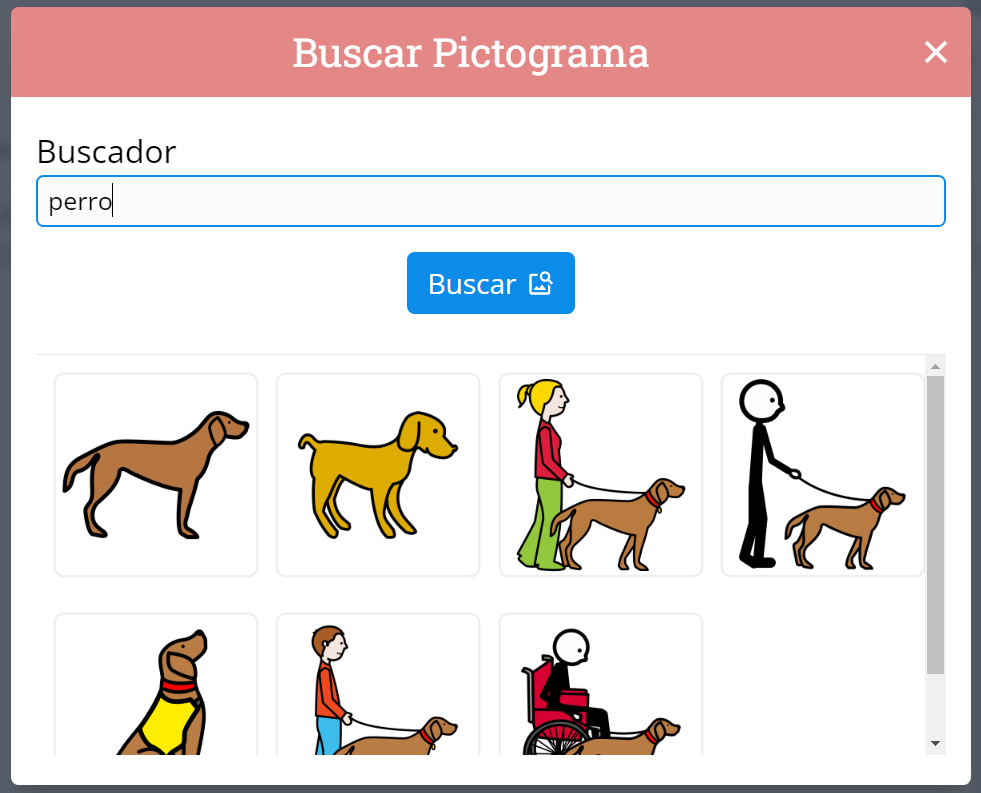
\includegraphics[width=0.7\textwidth]{Funcionalidades/BuscarPicto.png}
  \caption{Funcionalidad de Buscar Pictograma.}
  \label{fig:buscarPictograma}
\end{figure}

\subsubsection{Completar huecos}
\label{sec:impcompletarhuecos}
Para implementar esta funcionalidad se ha empleado un área de texto en la cual se introduce el texto que se quiere usar para crear los huecos. Tanto el botón de añadir huecos como el botón de \textit{Ok} están desactivados y no se podrán pulsar hasta que se introduzca un texto. Al pulsar el botón de añadir huecos, se permite hacer clic izquierdo en las distintas palabras del texto para convertirlas en huecos, y viceversa, pero no se podrá editar el texto. Se podrá editar el texto volviendo a pulsar el botón de añadir huecos, que ahora se llamará editar texto. Si se edita el texto se perderán todos los huecos que se hayan añadido. Además, se podrá elegir el tamaño de los huecos utilizando botones de radio. El usuario podrá elegir entre tamaño pequeño, mediano o grande para los huecos, siendo el tamaño mediano el valor por defecto. Al pulsar el botón de \textit{Ok}, se insertará en el documento de trabajo el ejercicio con el enunciado ``Resuelve el siguiente ejercicio completando los huecos con las palabras adecuadas:'' y el texto con los huecos que se hayan definido. En la Figura \ref{fig:impcompletarhuecos} se muestra la funcionalidad de completar huecos.

\begin{figure}[ht!]
  \centering
  \begin{subfigure}{\textwidth}
    \centering
    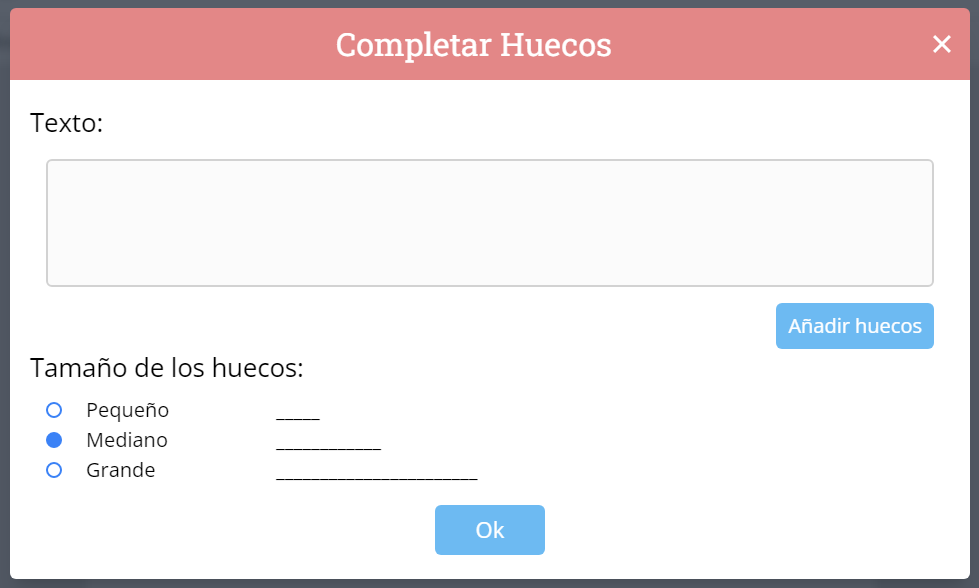
\includegraphics[width=0.7\textwidth]{Funcionalidades/CompletarHuecos01.png}
    \caption{Funcionalidad de completar huecos sin texto}
    \label{fig:impcompletarhuecos01}
  \end{subfigure}

  \begin{subfigure}{\textwidth}
    \centering
    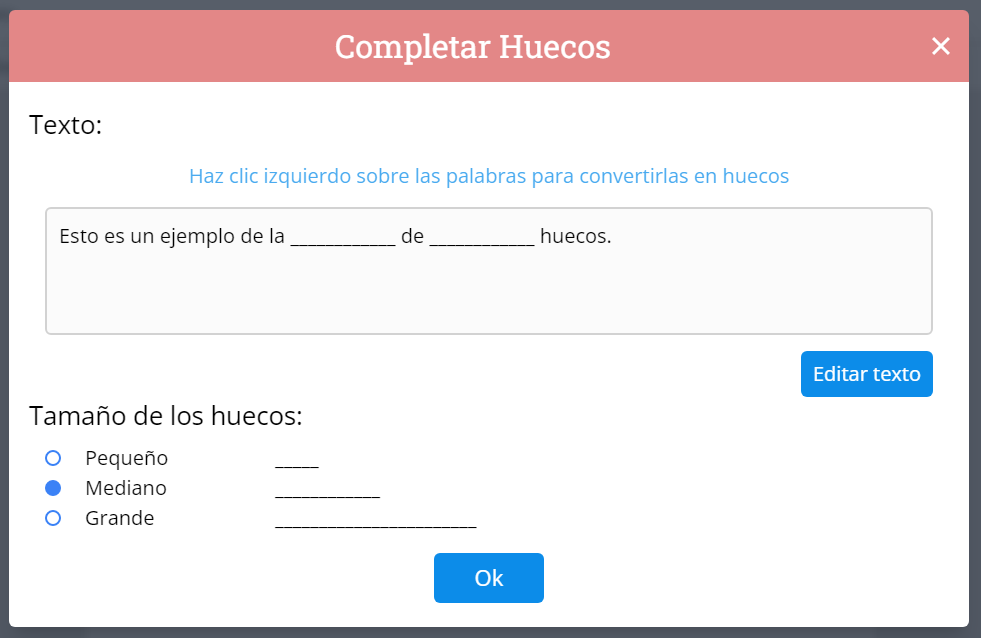
\includegraphics[width=0.7\textwidth]{Funcionalidades/CompletarHuecos02.png}
    \caption{Funcionalidad de completar huecos tras añadir huecos}
    \label{fig:impcompletarhuecos02}
  \end{subfigure}

  \begin{subfigure}{\textwidth}
    \centering
    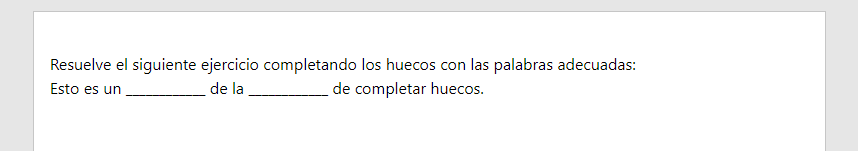
\includegraphics[width=0.7\textwidth]{Funcionalidades/CompletarHuecos03.png}
    \caption{Funcionalidad de completar huecos en documento de trabajo}
    \label{fig:impcompletarhuecos03}
  \end{subfigure}

  \caption{Funcionalidad de completar huecos}
  \label{fig:impcompletarhuecos}
\end{figure}

\subsubsection{Ejercicio de definiciones}
Cuando seleccionamos esta opción se nos despliega la interfaz de la Figura \ref{fig:funcionalidadDefinicion}. Para crear este tipo de ejercicio se debe rellenar el campo de conceptos a definir, que contiene los conceptos que se quieren definir. Se deben introducir en la entrada de texto que se posiciona debajo del título Conceptos, y  se pueden introducir al pulsar  la tecla \textit{ENTER} o presionando el botón con el icono del ``+''. En caso de querer borrar el concepto añadido se deberá presionar el botón con el icono de la papelera y si se quiere modificar se deberá presionar al boton con el icono del lápiz.
Una vez introducidos los conceptos a definir se habilitará el botón \textit{Ok}. Los otros campos son opcionales debido a tener valores por defecto. Estos son:
\begin{itemize}
  \item Tipos de pauta: Permite seleccionar la pauta que irá con cada concepto. El usuario podrá elegir entre espacio para dibujar, cuadrado para dibujar, doble pauta, pauta simple y cuadrícula. Por defecto es doble pauta.
  \item Número de filas: Se refiere a la cantidad de veces que se mostrará la pauta seleccionada. Su valor mínimo es de uno y máximo de cien. El valor por defecto es de una fila.
\end{itemize}
\begin{figure}[ht!]
  \centering
  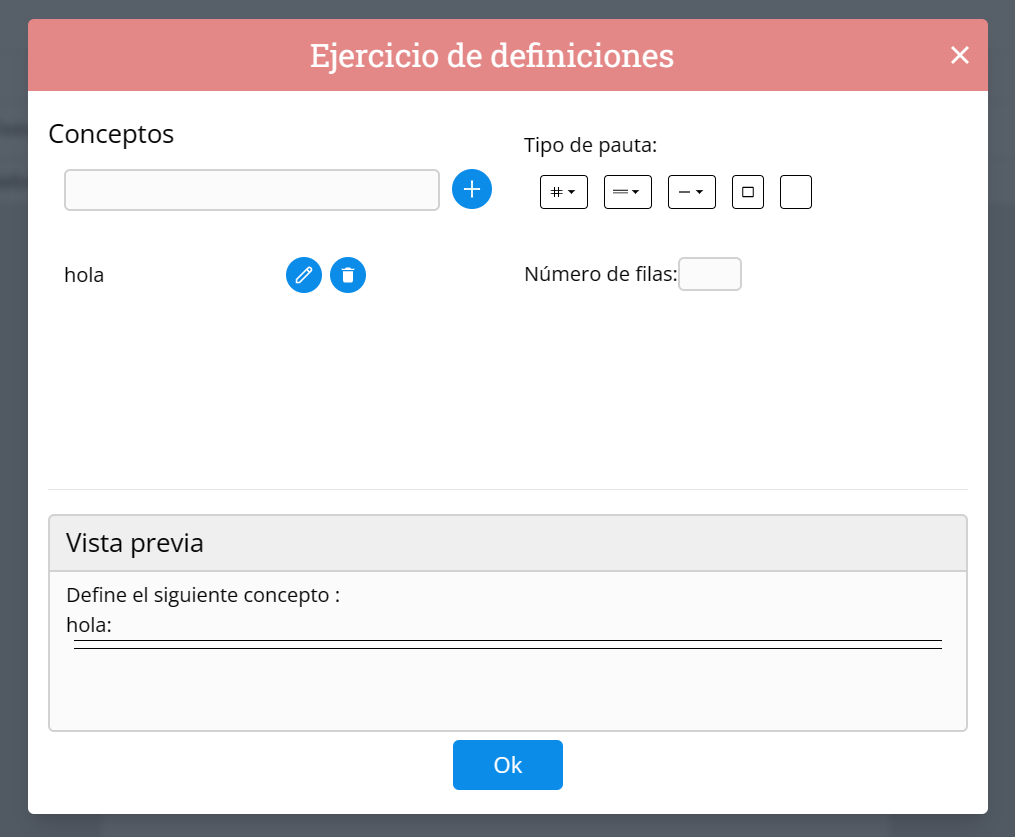
\includegraphics[width=0.7\textwidth]{Imagenes/Funcionalidades/EjercicioDefinicion.png}
  \caption{Funcionalidad de definición.}
  \label{fig:funcionalidadDefinicion}
\end{figure}
Cabe mencionar que el campo de Tipos de pauta emplea una botonera que se repite en otros ejercicios. Para reutilizarla se ha optado por desacoplarla y abstraerla en un componente separado. Este componente permite al usuario seleccionar los botones de pauta deseados. Además, recibe un estado donde introduce la opción elegida.
Para lograr esto, se ha utilizado el patrón \textit{Factory}. De esta manera se puede crear el componente de botonera de pautas adaptándolo a cada uno de los ejercicios en los que se utilizará.

\subsubsection{Ejercicio de Desarrollo}
\label{sec:impdesarrollo}
Esta funcionalidad permite crear un ejercicio de desarrollo en el que hay un enunciado y un espacio en el que el estudiante puede desarrollar su respuesta. Dependiendo del tipo de respuesta esperada, se pueden insertar diferentes tipos de espacios para contestar, por ejemplo, pauta simple, doble pauta, espacio para dibujar, etc. En la Figura \ref{fig:funcionalidadDesarrollo} se muestra el modal en el que se puede crear el ejercicio.

Para implementar esta funcionalidad se han usado varios elementos como un campo de texto para escribir el enunciado, un campo para indicar el número de líneas que se quiere insertar y un selector para elegir el tipo de pauta que se quiere utilizar. Por defecto, los valores que tiene son una fila de doble pauta. El selector de tipo de pauta consta de 5 botones con diferentes opciones, como cuadrícula, pauta simple, doble pauta, recuadro y espacio en blanco. En la funcionalidad anterior se explica la abstracción de los botones utilizados para las pautas.

\begin{figure}[ht!]
  \centering
  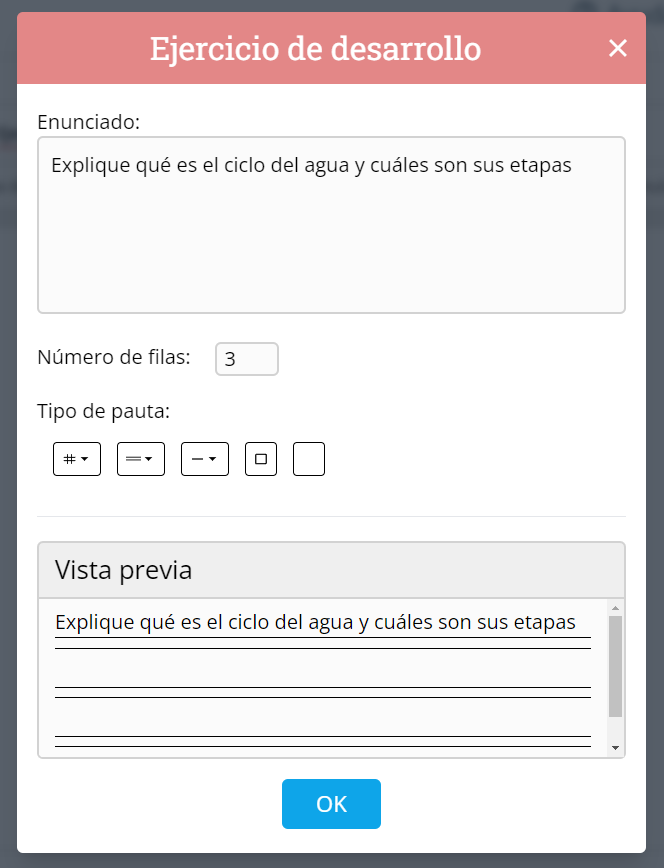
\includegraphics[width=0.7\textwidth]{Imagenes/Funcionalidades/DesarrolloModal.PNG}
  \caption{Funcionalidad de ejercicios de desarrollo.}
  \label{fig:funcionalidadDesarrollo}
\end{figure}

\subsubsection{Ejercicio de fórmulas matemáticas}
\label{sec:impmatematica}
Esta funcionalidad permite crear un ejercicio de fórmulas matemáticas en el que los alumnos deberán rellenar los espacios en blanco indicados por el profesor para completar la expresión. Se pueden añadir varias fórmulas en el mismo ejercicio y estas aparecerán enumeradas. En la Figura \ref{fig:funcionalidadFormulaMatematica} se muestra el modal en el que se puede crear el ejercicio.

Para implementar esta funcionalidad se han usado una serie de campos de texto, los cuales representan cada elemento de la fórmula matemática. Un campo vacío representa un hueco que debe ser rellenado por el alumno. En el estado de \textit{MathFormulaModal} se guarda un array llamado fórmulas, en el que se almacena cada fórmula matemática, las cuales también son arrays que contienen cada elemento. Este array se ve reflejado en la vista, cada fórmula se muestra en una fila diferente y todos sus elementos se representan usando campos de texto que el usuario puede editar.

Cuando el usuario presiona una tecla, se comprueba si ha presionado el espacio, el \textit{backspace} o el \textit{enter}. En caso de haber presionado la tecla de espacio, el array se modifica para insertar una nueva casilla en la posición siguiente a la actual. Esto se ve reflejado en la vista al añadirse un nuevo campo de texto. En caso de haber presionado la tecla de \textit{backspace}, si el \textit{input} actual está vacío, esta posición se eliminará del array, lo cual causa que este campo de texto también desaparezca de la interfaz. También, si se presiona el \textit{backspace} y se elimina el último elemento de la fila, esta fórmula se eliminará. Por último, al presionar la tecla de \textit{enter} se añade una nueva fórmula matemática vacía. El usuario también puede añadir o eliminar fórmulas haciendo clic en los botones que se muestran en el modal.
Al presionar el botón de \textit{Ok}, simplemente se insertan todas las fórmulas matemáticas, el texto de cada casilla estará separado por un espacio, y en las posiciones que se encuentren vacías se inserta una línea indicando el hueco que el alumno deberá rellenar. 

\begin{figure}[ht!]
  \centering
  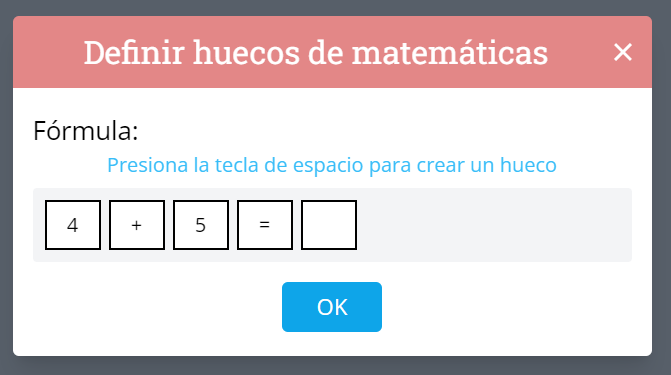
\includegraphics[width=0.7\textwidth]{Imagenes/Funcionalidades/MathFormulaModal.PNG}
  \caption{Funcionalidad de fórmula matemática.}
  \label{fig:funcionalidadFormulaMatematica}
\end{figure}

\subsubsection{Sopa de letras}
\label{sec:impsopaletras}
Para la generación de la sopa de letras se utiliza la biblioteca \textit{word-search}\footnote{\url{https://www.npmjs.com/package/@blex41/word-search}}. Esta biblioteca permite crear sopas de letras mediante la clase \textit{WordSearch}, que requiere un objeto con las distintas opciones de la sopa de letras. En el Listing \ref{fig:impsopaletrasopciones} se muestra un ejemplo de las opciones y de como se crea la sopa de letras. La clase \textit{WordSearch} contiene distintos atributos y funciones para obtener información sobre la sopa de letras. Los dos atributos que se han utilizado en este proyecto son \textit{grid}, que contiene la sopa de letras en forma de matriz, y \textit{words}, que contiene las palabras que se han incluido en la sopa de letras.

\begin{lstlisting}[label=fig:impsopaletrasopciones, caption=Opciones para la sopa de letras., language=JavaScript, float]
  // Hay mas opciones pero estas son las basicas
  // Si falta alguna opcion, se le dara un valor por defecto
  const options = {
    // Numero de columnas de la sopa de letras
    cols: 6,
    // Numero de filas de la sopa de letras
    rows: 6,
    // Orientaciones no permitidas (N, E, S, W, NE, SE, SW, NW)
    disabledDirections: ["N", "W", "NW", "SW"],
    // Numero maximo de palabras que pueden aparecer en la sopa de letras
    maxWords: 20,
    // Palabras que deben aparecer en la sopa de letras
    // Dependiendo de las dimensiones, orientaciones
    // y numero maximo de palabras puede que no aparezcan todas
    dictionary: ["Hello", "crepe", "Skoda", "word", "search"],
    // Probabilidad de que las palabras aparezcan al reves
    backwardsProbability: 0.3,
    // Letras en mayusculas
    upperCase: true,
    // Permitir tildes diacriticas
    diacritics: true
  };

  // Generar la sopa de letras con las opciones anteriores
  const ws = new WordSearch(options);
\end{lstlisting}

Para implementar esta funcionalidad se emplean dos campos para introducir el número de filas y columnas deseado. A continuación, se utilizan dos componentes, el \textit{ModalNewWordInput} y el \textit{ModalWordList}, que permiten añadir, modificar y eliminar palabras de la sopa de letras. Para seleccionar las orientaciones permitidas se ha creado un menú de \textit{checkboxes}. Cada vez que se modifica alguno de estos campos se llama a la función \textit{createWordSearch}, que utiliza la clase \textit{WordSearch} de la biblioteca \textit{word-search} para generar la sopa de letras. Esta función recibe los valores de los campos del modal y devuelve un objeto que contiene la sopa de letras (la matriz \textit{grid} de la clase \textit{WordSearch}), una lista de errores y una lista de avisos. En caso de que haya algún error, no se generará la sopa de letras y, por lo tanto, esta y los avisos serán nulos. La sopa de letras generada se muestra en una vista previa, y si hay errores o avisos, se muestran en una alerta en la parte superior de la vista previa. Al pulsar el botón de \textit{Ok}, se insertará un ejercicio en el documento de trabajo, con un enunciado especificando las distintas palabras o el número de palabras a buscar y las posibles orientaciones de estas, y debajo de este se insertará la sopa de letras, centrada en la página. En la Figura \ref{fig:impsopaletras} se muestra la funcionalidad completa de la sopa de letras.

\begin{figure}[ht!]
  \centering
  \begin{subfigure}{\textwidth}
    \centering
    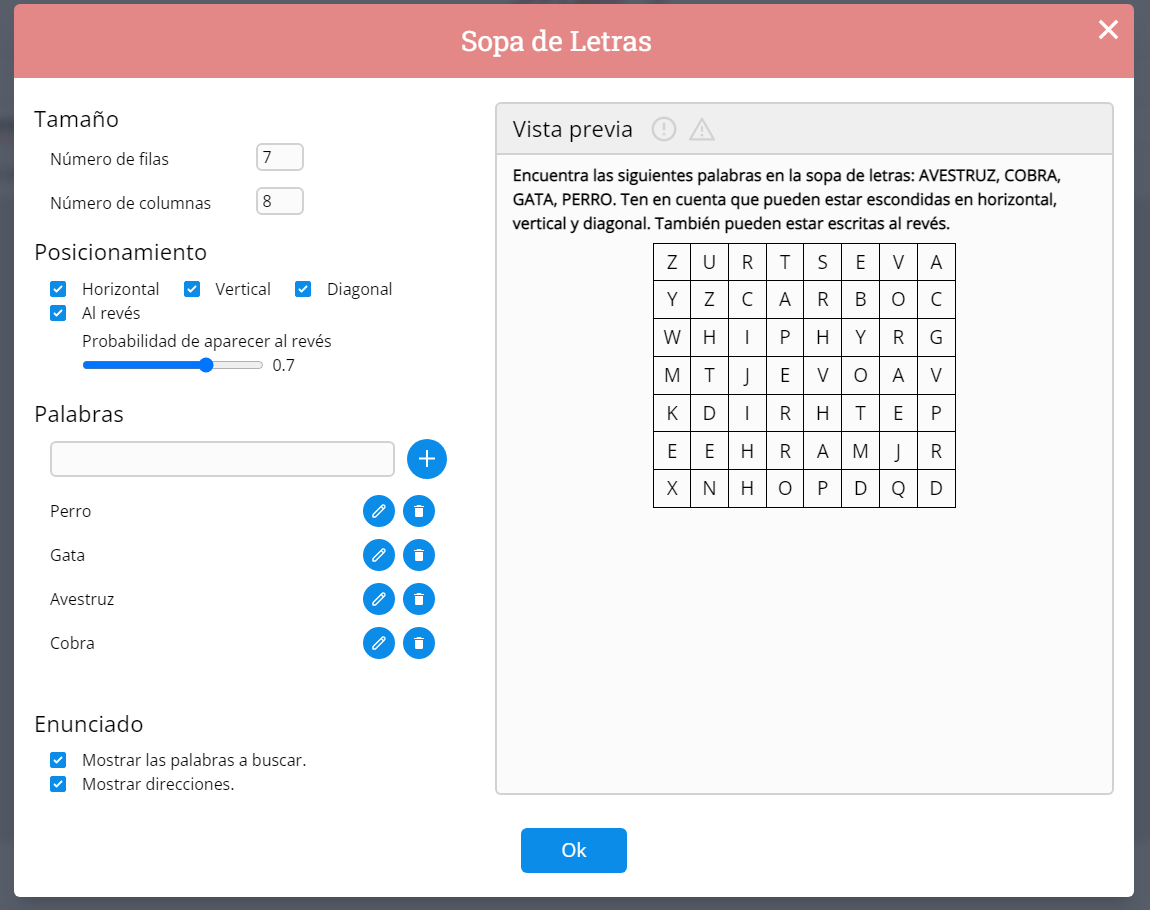
\includegraphics[width=0.7\textwidth]{Funcionalidades/SopaLetras01.png}
    \caption{Ventana modal de la funcionalidad de sopa de letras}
    \label{fig:impsopaletras01}
  \end{subfigure}

  \begin{subfigure}{\textwidth}
    \centering
    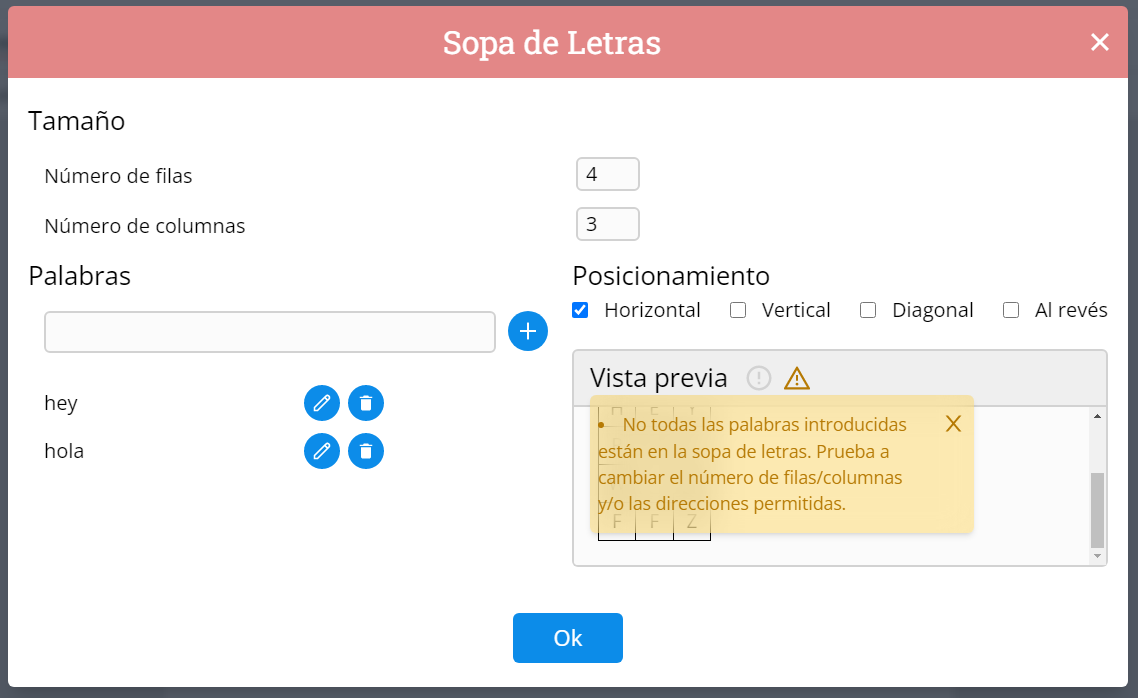
\includegraphics[width=0.7\textwidth]{Funcionalidades/SopaLetras02.png}
    \caption{Ejemplo, en el documento de trabajo, de la funcionalidad de sopa de letras}
    \label{fig:impsopaletras02}
  \end{subfigure}

  \caption{Funcionalidad de sopa de letras}
  \label{fig:impsopaletras}
\end{figure}

\subsubsection{Ejercicio de verdadero/falso}
\label{sec:funcioVF}
Para esta funcionalidad se ha utilizado un campo de texto en el cual se introducen las frases del ejercicio. Al darle a la tecla \textit{ENTER} se introducirán dichas frases debajo del campo de texto y se guardarán en una lista. Se proporcionan dos opciones para editar las frases: eliminar (representado por un icono de basura) o modificar (representado por un icono de lápiz).

La vista previa se genera automáticamente y muestra el enunciado del ejercicio ``Responde Verdadero o Falso según corresponda.'' junto con las frases y un cuadrado. El botón de ``Reordenar'' aparecerá cuando haya más de dos frases en la vista previa. Para reordenar las frases, se aplica el algoritmo Sattolo Cycle\footnote{\url{https://rosettacode.org/wiki/Sattolo_cycle}} a una lista distinta de la inicial donde se encuentran todas las frases. Este algoritmo reorganiza los elementos de una lista de forma aleatoria, pero sin repetir el mismo elemento en la misma posición dos veces seguidas.

Una vez que el usuario ha terminado de editar las frases, se puede enviar el ejercicio al documento de trabajo presionando el botón \textit{Ok}, el cual está inhabilitado al ingresar al modal. En la Figura \ref{fig:veryfalso} se muestra la funcionalidad de verdadero y falso.

\begin{figure}[ht!]
  \centering
  \begin{subfigure}{\textwidth}
    \centering
    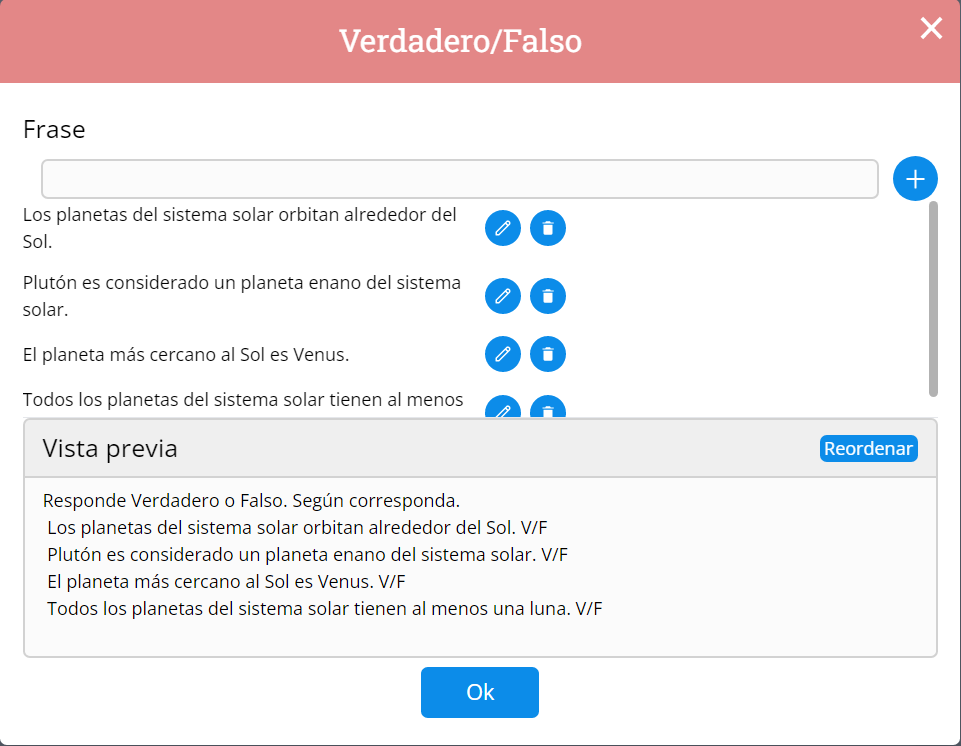
\includegraphics[width=0.7\textwidth]{Funcionalidades/VyF.PNG}
    \caption{Ventana modal de la funcionalidad de verdadero y falso.}
    \label{fig:vyf}
  \end{subfigure}

  \begin{subfigure}{\textwidth}
    \centering
    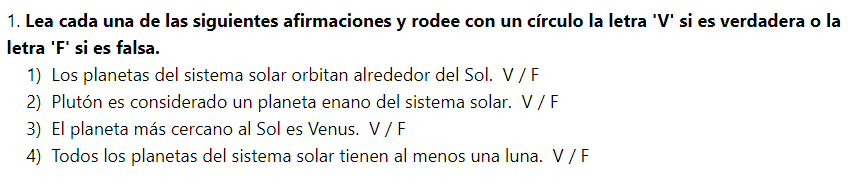
\includegraphics[width=0.7\textwidth]{Funcionalidades/VyFEditor.PNG}
    \caption{Ejemplo, en el documento de trabajo, de la funcionalidad de verdadero y falso.}
    \label{fig:vyfEdit}
  \end{subfigure}

  \caption{Funcionalidad de verdadero y falso}
  \label{fig:veryfalso}
\end{figure}


\subsubsection{Generar resumen}
\label{sec:impresumen}
Para implementar esta funcionalidad se ha empleado un área de texto en la cual se introduce el texto que se quiere resumir. Tanto el botón de resumir como el botón de \textit{Ok} están desactivados por defecto. El botón de resumir se activará cuando el usuario introduzca un texto para resumir, mientras que el botón de \textit{Ok} se activará cuando haya un resumen válido. Para seleccionar el número de palabras aproximado que debe tener el resumen se ha utilizado un ``tirador'' o control deslizante.

Para generar el resumen se ha utilizado la API que proporciona \textit{OpenAI}\footnote{\url{https://platform.openai.com/overview}}. Esta API proporciona acceso a modelos de inteligencia avanzados desarrollados por \textit{OpenAI}\footnote{\url{https://openai.com/product}}. Estos modelos están diseñados para procesar y generar texto, imágenes, sonidos y otros tipos de datos. Para implementar esta funcionalidad se ha utilizado el modelo GPT-3. Este modelo es el que utiliza actualmente \textit{ChatGPT}\footnote{\url{https://openai.com/blog/chatgpt}} y puede generar texto coherente y relevante a partir de una breve descripción proporcionada por el usuario. Para poder utilizar esta API se pueden realizar distintas peticiones HTTP, pero si se utiliza \textit{Node.js} se puede instalar el paquete \textit{openai}\footnote{\url{https://www.npmjs.com/package/openai}}. Este paquete proporciona la clase \textit{OpenAIApi}, la cual permite utilizar distintas funciones que realizan las peticiones HTTP necesarias. En el Listing \ref{fig:impresumenconfiguracion} se muestra la configuración de la clase \textit{OpenAIApi}. La función \textit{createChatCompletion} permite simular un chat con un modelo de procesamiento de texto. Esta función recibe como entrada el modelo que se quiere utilizar, y una lista de mensajes. Cada mensaje esta compuesto por el rol del autor (\textit{system}, \textit{assistant} y \textit{user}) y el contenido del mensaje (\textit{prompt}). La función \textit{createChatCompletion} devuelve un objeto con información sobre la conversación y las distintas respuestas generadas a partir de los mensajes que se han enviado.

\begin{lstlisting}[label=fig:impresumenconfiguracion, caption=Configuración de la clase \textit{OpenAIApi}., language=JavaScript]
  const { Configuration, OpenAIApi} = require("openai");

  const configuration = new Configuration({
    apiKey: "Clave de la API (se necesita una cuenta de OpenAI)."
  });

  const openai = new OpenAIApi(configuration);
\end{lstlisting}

Al pulsar el botón de resumir se realiza una petición HTTP de tipo POST a la ruta ``/summary'', enviando el texto a resumir y el número de palabras del resumen. En el \textit{backend} se llama a la función \textit{createChatCompletion} de la clase \textit{OpenAIApi}, utilizando ``Resume este texto en aproximadamente \{número de palabras\} palabras, si no se puede resumir el texto devuelve -1: \{texto original\}'' como \textit{prompt}, con el número de palabras y el texto introducidos por el usuario, y se devuelve el resumen generado al cliente. El resumen se mostrará en el panel de vista previa. En caso de que no se pueda generar el resumen, o el texto original sea muy breve, se mostrará un error al usuario en la vista previa. Al pulsar el botón de \textit{Ok}, se cerrará el modal y se insertará el texto resumido en el documento de trabajo. En la Figura \ref{fig:impresumen} se muestra la funcionalidad de generar resumen.

\begin{figure}[ht!]
  \centering
  \begin{subfigure}{\textwidth}
    \centering
    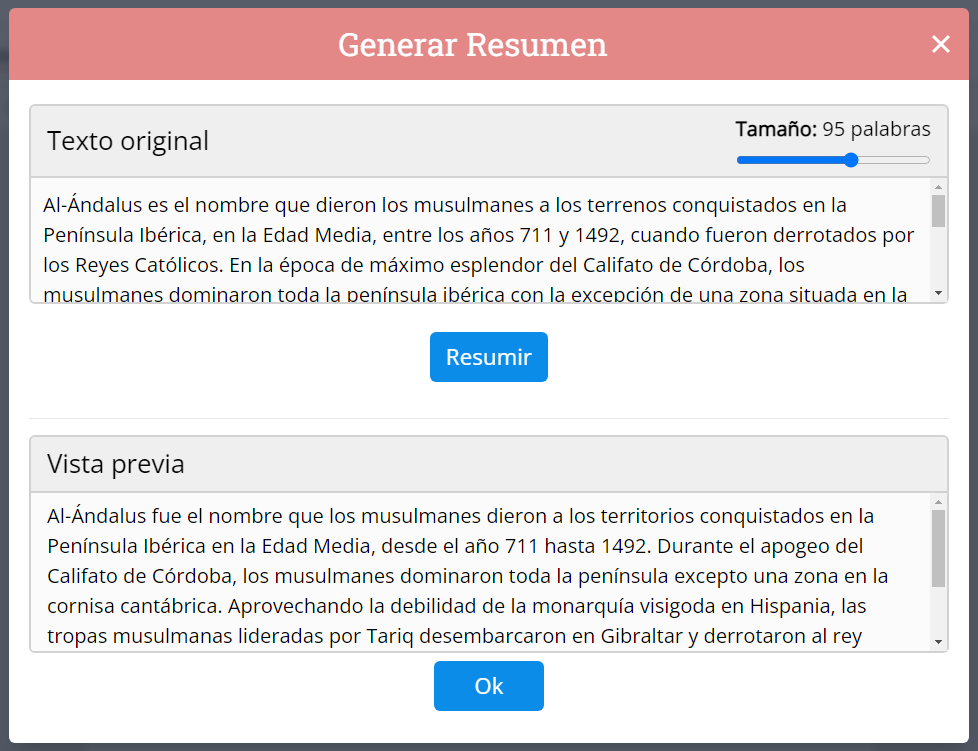
\includegraphics[width=0.7\textwidth]{Funcionalidades/Resumen01.png}
    \caption{Ventana modal de la funcionalidad de generar resumen}
    \label{fig:impresumen01}
  \end{subfigure}

  \begin{subfigure}{\textwidth}
    \centering
    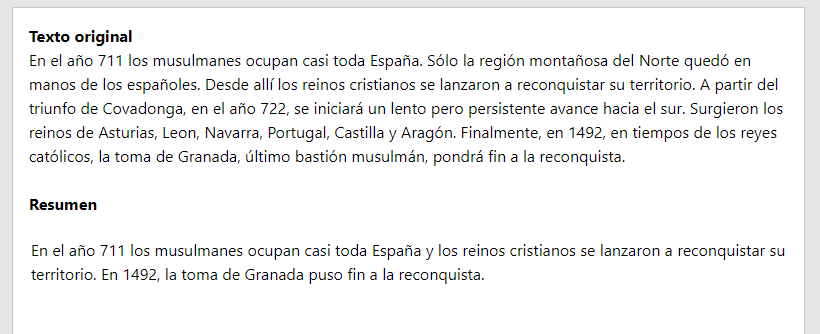
\includegraphics[width=0.7\textwidth]{Funcionalidades/Resumen02.png}
    \caption{Ejemplo, en el documento de trabajo, de la funcionalidad de generar resumen}
    \label{fig:impresumen02}
  \end{subfigure}

  \caption{Funcionalidad de generar resumen}
  \label{fig:impresumen}
\end{figure}

\subsubsection{Leyenda de colores}
\label{sec:leyendaColores}
Para implementar esta funcionalidad se han utilizado dos campos de texto, en uno se introduce el título de la leyenda de colores y en otro los conceptos. Para cada concepto se ha asignado un color mediante un campo de entrada de color. Tanto los colores como los conceptos se almacenan en una lista. Se proporcionan dos opciones para editar tanto los conceptos como los colores asociados: eliminar (representado por un icono de basura) o modificar (representado por un icono de lápiz).

La vista previa se genera automáticamente y muestra el título de la leyenda de colores junto con los conceptos y su respectivo color. Al pulsar el botón \textit{Ok} se envía la leyenda de colores al editor de trabajo, dicho botón se encuentra inhabilitado al ingresar al modal. En la Figura \ref{fig:leyendacolor} se muestra la funcionalidad de leyenda de colores.

\begin{figure}[ht!]
  \centering
  \begin{subfigure}{\textwidth}
    \centering
    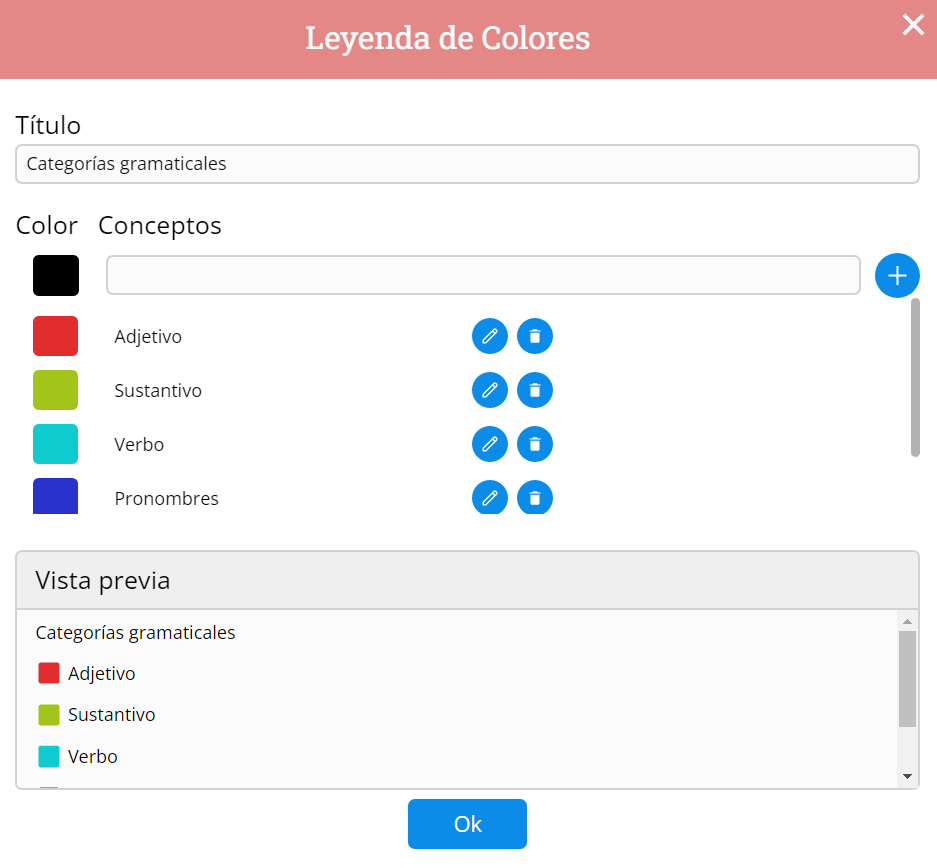
\includegraphics[width=0.7\textwidth]{Funcionalidades/LeyendaColor.PNG}
    \caption{Ventana modal de la funcionalidad de leyenda de colores}
    \label{fig:leyendacolor01}
  \end{subfigure}

  \begin{subfigure}{\textwidth}
    \centering
    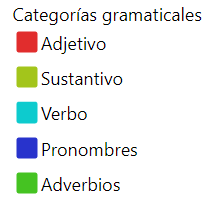
\includegraphics[width=0.5\textwidth]{Funcionalidades/LeyendaColor2.PNG}
    \caption{Ejemplo, en el documento de trabajo, de la funcionalidad de leyenda de colores}
    \label{fig:leyendacolor02}
  \end{subfigure}

  \caption{Funcionalidad de leyenda de colores}
  \label{fig:leyendacolor}
\end{figure}

\subsubsection{Pictotraductor}
\label{sec:imppictotraductor}
Para implementar esta funcionalidad se ha empleado un área de texto en la cual se introduce el texto que se quiere traducir a pictogramas. El botón de traducir está desactivado por defecto, mientras que el botón de \textit{Ok} no apecerá hasta que se haya traducido el texto a pictogramas. El botón de traducir se activará cuando el usuario introduzca texto para traducir. Al traducir el texto, si no se ha encontradon pictogramas, se mostrará ``No se han encontrado pictogramas'' y no se mostrará el botón de \textit{Ok}. Si se encuentran pictogramas, estos se mostrarán en formato cuadrícula, con la palabra a la que se asocian encima. Como una palabra puede tener varios pictogramas asociados, cada pictograma dispone de dos botones en los laterales, en forma de flecha, que se pueden utilizar para cambiar el pictograma asociado a esa palabra. También hay un botón debajo de cada pictograma para esconderlo. El botón de \textit{Ok} se activará cuando haya al menos un pictograma visible. Para configurar los pictogramas, se dispone de un menu desplegable en el cual se puede seleccionar el posicionamiento de la palabra asociada al pictograma (arriba, abajo, sin texto) y marcar si se quieren los pictogramas en blanco y negro o en color.

Cuando se pulsa el botón de traducir se realiza una petición HTTP de tipo POST al servidor \textit{backend}, a la ruta ``/pictotranslator'', enviando el texto introducido por el usuario. En el \textit{backend}, se extraen todas las palabras del texto y se realiza una petición a la API de ARASAAC por cada una para obtener los pictogramas relacionados con esa palabra. El servidor devuelve al cliente un objeto \textit{JSON} con la palabra, los pictogramas asociados a esta, si el pictograma está desactivado y que pictograma está seleccionado.

Al pulsar el botón de \textit{Ok}, se cerrará el modal y se insertará el texto traducido en el documento de trabajo. Las palabras que no tuviesen pictogramas y las palabras cuyo pictograma ha sido desactivado por el usuario, se mostrarán sin pictograma. En la Figura \ref{fig:imppictotraductor} se muestra la funcionalidad de pictotraductor.

\begin{figure}[ht!]
  \centering
  \begin{subfigure}{\textwidth}
    \centering
    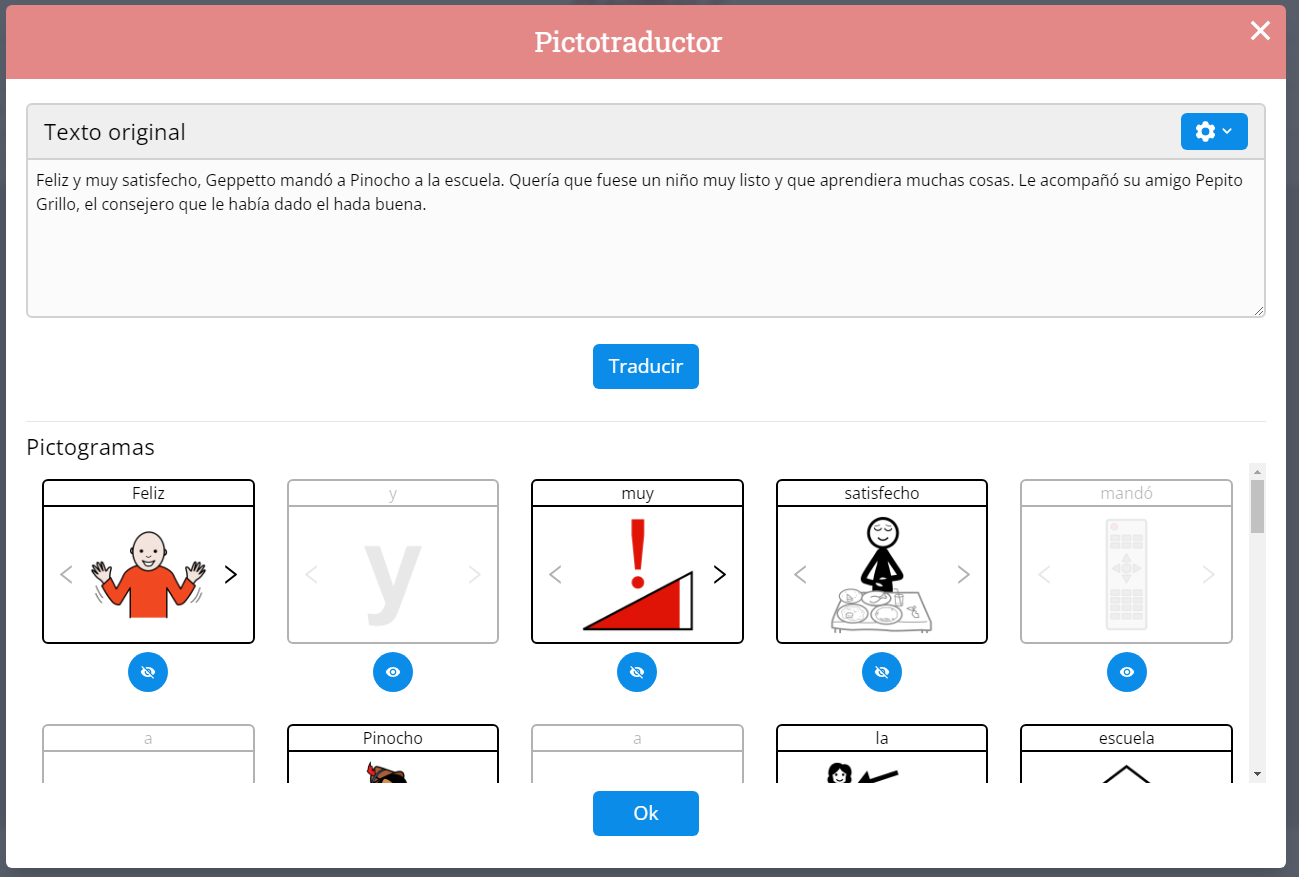
\includegraphics[width=0.7\textwidth]{Funcionalidades/Pictotraductor01.png}
    \caption{Ventana modal de la funcionalidad de pictotraductor}
    \label{fig:imppictotraductor01}
  \end{subfigure}

  \begin{subfigure}{\textwidth}
    \centering
    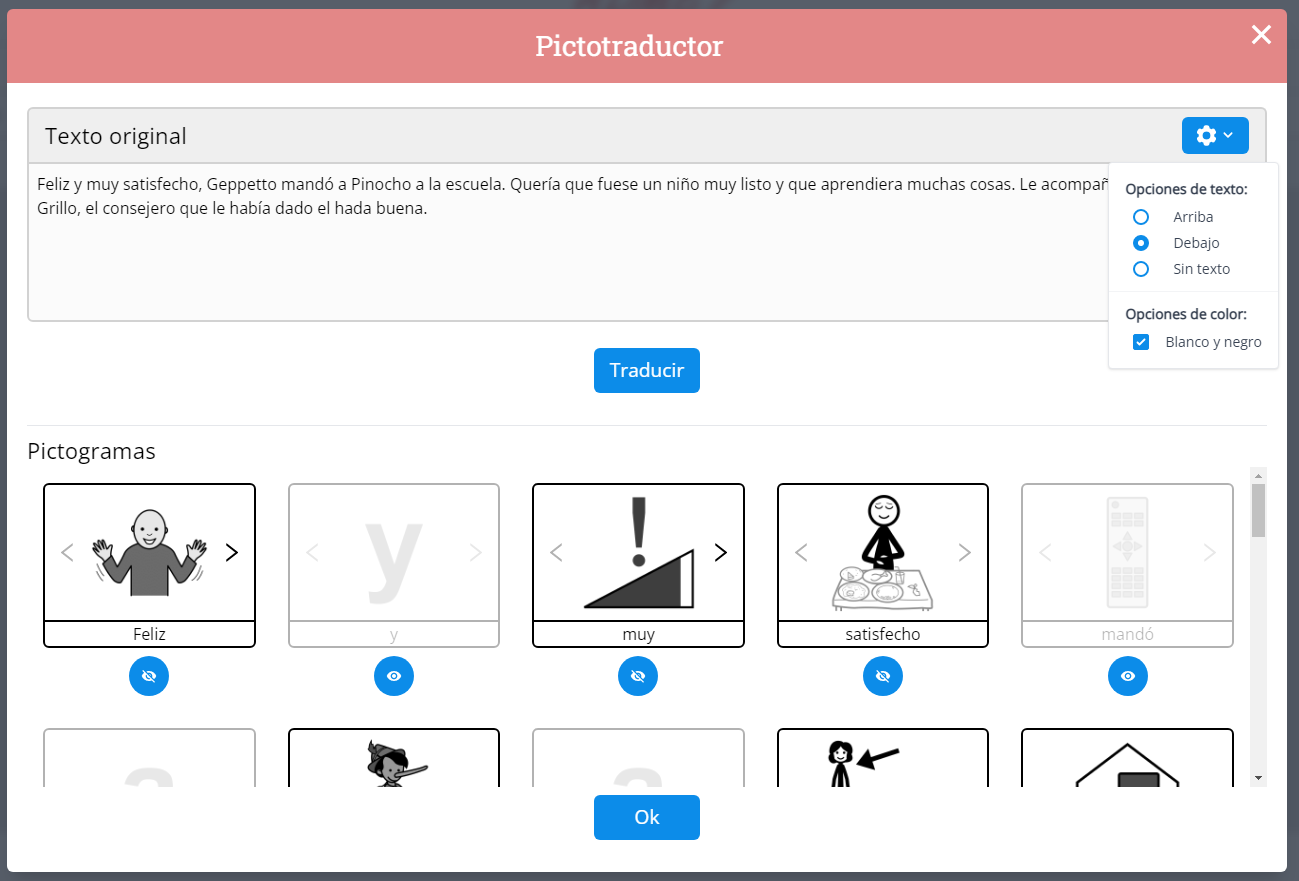
\includegraphics[width=0.7\textwidth]{Funcionalidades/Pictotraductor02.png}
    \caption{Configuración de los pictogramas de la funcionalidad de pictotraductor}
    \label{fig:imppictotraductor02}
  \end{subfigure}

  \begin{subfigure}{\textwidth}
    \centering
    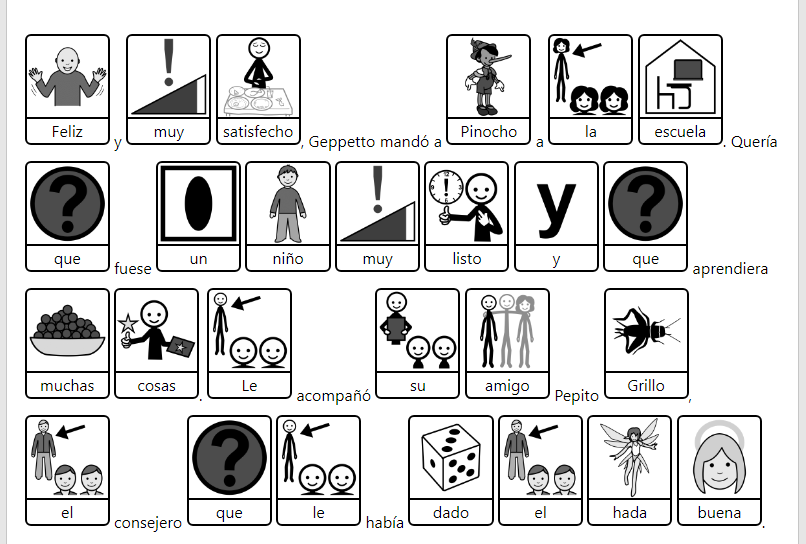
\includegraphics[width=0.7\textwidth]{Funcionalidades/Pictotraductor03.png}
    \caption{Ejemplo, en el documento de trabajo, de la funcionalidad de pictotraductor}
    \label{fig:imppictotraductor03}
  \end{subfigure}

  \caption{Funcionalidad de pictotraductor}
  \label{fig:imppictotraductor}
\end{figure}


\subsubsection{Ejercicio de Espacio Para Dibujar}
\label{sec:impespacioparadibujar}
Esta funcionalidad permite crear un ejercicio en el que hay un enunciado y un espacio en blanco en el que el alumno puede realizar un dibujo basándose en lo que pide el profesor. El tamaño de este espacio es personalizable y también se puede indicar si se quiere mostrar un borde para delimitarlo o no. En la Figura \ref{fig:funcionalidadEspacioParaDibujar} se muestra el modal en el que se puede crear el ejercicio.

Para implementar esta funcionalidad se han usado varios elementos como un campo de texto para escribir el enunciado, un campo para indicar el tamaño del espacio que se quiere insertar y un \textit{checkbox} para seleccionar si el espacio para dibujar debe tener un recuadro o no. En este caso, el recuadro es simplemente un borde negro alrededor del espacio. Por último, hay una vista previa en la que se puede observar cómo se verá el ejercicio una vez que se inserte en el editor de texto. Por defecto, el valor del tamaño del espacio es 1 centímetro de alto y el \textit{checkbox} está marcado, indicando que sí se debe mostrar el recuadro.

Una vez introducidos un enunciado y un tamaño válidos, se habilitará el botón de \textit{Ok} para poder insertar el ejercicio en el documento de trabajo.


\begin{figure}[ht!]
  \centering
  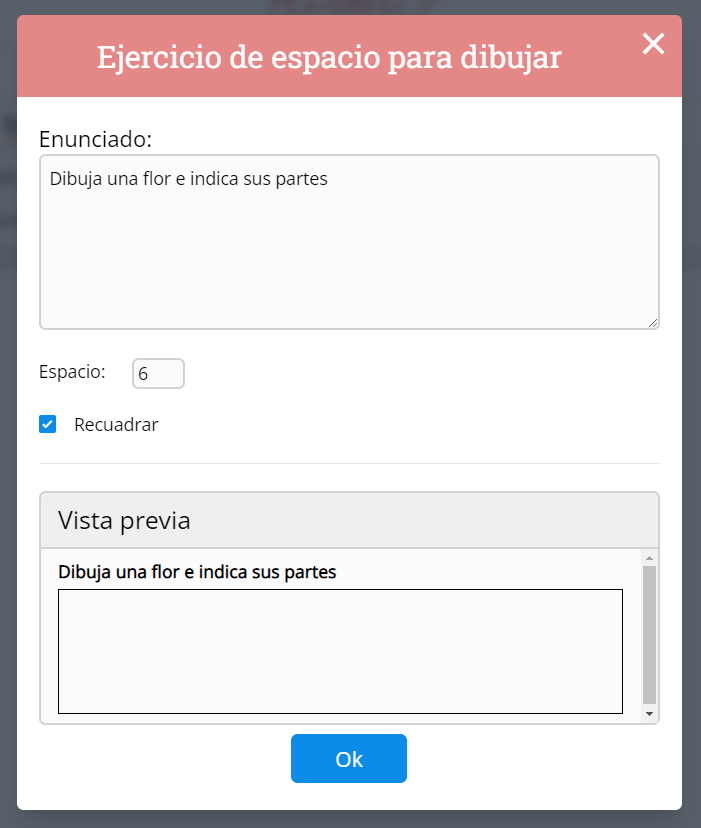
\includegraphics[width=0.7\textwidth]{Imagenes/Funcionalidades/EspacioParaDibujar.PNG}
  \caption{Funcionalidad de espacio para dibujar.}
  \label{fig:funcionalidadEspacioParaDibujar}
\end{figure}



\subsection{Del modal al editor}
En el proceso de inserción del resultado obtenido en la ventana modal en el editor de texto con Slate, creamos un nodo específico para almacenar la información correspondiente. Después de que el usuario ha confirmado el resultado del modal presionando el botón \textit{Ok}, creamos un nodo específico que se encarga de transferir este contenido al documento. Luego, utilizamos la función \textit{insertNode} de Slate para agregar este nodo al área editable, lo que nos permite integrar el contenido del modal con el resto del documento.

Además de esto, hemos utilizado plugins definidos para mejorar aún más la integración del contenido del modal en el documento. Estos plugins nos permiten personalizar la forma en que se maneja y se presenta el contenido, lo que nos da una mayor flexibilidad.

